% Memoria del proyecto SaaS de votación digital.
% Basada en la especificación de requisitos versión 1.0 (07/10/2026).

\chapter{Introducción}
\label{cap:introduccion}

Las universidades, asociaciones y comunidades necesitan procesos de votación
que permitan gestionar el censo, emitir votos y publicar resultados de forma
comprensible y verificable. En la práctica, algunas organizaciones combinan
hojas de cálculo, formularios genéricos y comunicaciones por correo. Ese
enfoque puede dificultar la comprobación de la identidad y elegibilidad de
quienes participan, la protección del secreto del voto y la auditoría del
escrutinio.

Este trabajo presenta el diseño e implementación de VeriVoto, una plataforma
de votación digital ofrecida como Software as a Service (SaaS). El prototipo
permite a distintas organizaciones configurar procesos electorales en una
infraestructura compartida con aislamiento lógico de sus datos. La memoria
documenta sus requisitos, arquitectura, implementación y evaluación disponible.

\section{Problema y motivación}
\label{sec:problema}

El flujo habitual comienza con la preparación manual del censo y de las
opciones de voto. Después, el organizador configura una herramienta externa y
envía enlaces por correo electrónico. El votante selecciona una opción, pero
puede no recibir evidencia de que el voto se registró correctamente. Al cierre,
el organizador obtiene un resultado cuya integridad y trazabilidad pueden ser
difíciles de comprobar por terceros.

La propuesta aborda estas limitaciones mediante controles de acceso, gestión
del ciclo de vida de la votación, separación entre identidad y urna, recibos de
verificación, registros de auditoría y una interfaz accesible. La verificación
debe presentarse de forma comprensible para personas sin conocimientos
criptográficos. La resistencia a la coacción y las garantías formales de
verificabilidad extremo a extremo requieren un análisis específico y se
consideran límites que deberán concretarse en el diseño.

\section{Objetivos}
\label{sec:objetivos}

El objetivo general es diseñar, implementar y evaluar un prototipo funcional
de plataforma SaaS de votación digital segura y auditable para organizaciones,
con arquitectura cloud multi-tenant y API abierta, que responda a los huecos
identificados en autenticación, experiencia móvil y verificación comprensible.
El prototipo y la evidencia de evaluación disponible se presentan en esta
memoria; las pruebas de integración, accesibilidad, carga y usabilidad siguen
pendientes. Los objetivos del sistema son:

\begin{description}
  \item[OBJ-1.] Implementar y documentar la arquitectura SaaS multi-tenant y la gestión de
  organizaciones, identidad, roles y permisos, con autenticación genérica.
  \item[OBJ-2.] Implementar y documentar la gestión del censo, la configuración y el ciclo de
  vida de votaciones, junto con una API abierta documentada.
  \item[OBJ-3.] Implementar un flujo de participación orientado a la accesibilidad que
  proteja el secreto y la unicidad y proporcione una evidencia comprensible.
  \item[OBJ-4.] Implementar el escrutinio, la trazabilidad y las actas, y evaluar
  la calidad conforme al modelo ISO/IEC 25010:2023 según la evidencia disponible.
\end{description}

\subsection{Objetivos específicos}
\label{sec:objetivos-especificos}

Los objetivos del sistema se concretan en los siguientes objetivos específicos
de implementación, documentación y evaluación:
\begin{description}
  \item[OE1.] Implementar y documentar la gestión multi-organización y el control de acceso
  mediante roles, permisos y aislamiento de datos.
  \item[OE2.] Implementar y documentar la gestión del censo y el ciclo de vida de los
  procesos, desde su configuración hasta el cierre.
  \item[OE3.] Implementar y evaluar el flujo de autenticación, emisión del voto y
  obtención y verificación de un recibo comprensible.
  \item[OE4.] Implementar y documentar el escrutinio, la publicación de resultados y las
  evidencias de auditoría que permitan revisar su integridad.
\end{description}

\section{Preguntas de investigación}
\label{sec:preguntas-investigacion}

\begin{description}
  \item[RQ1.] ¿Cómo puede una plataforma SaaS garantizar la verificación del
  voto de forma comprensible para usuarios no técnicos?
  \item[RQ2.] ¿Qué mecanismos de separación de identidad y urna permiten
  proteger el secreto del voto y controlar la unicidad de la participación?
  \item[RQ3.] ¿Cómo se puede evaluar la calidad del producto software
  resultante tomando ISO/IEC 25010:2023 como modelo de referencia?
\end{description}

\section{Trazabilidad de objetivos, preguntas y evaluación}
\label{sec:trazabilidad-investigacion}

La tabla~\ref{tab:trazabilidad-investigacion} conecta cada objetivo
específico con las preguntas que aborda, los casos de uso implicados y las
evidencias de calidad que se proponen para evaluarlo. Los umbrales son los
recogidos en los RNF del proyecto y siguen pendientes de validación.

\small
\setlength{\tabcolsep}{3.5pt}
\begin{longtable}{|p{0.08\textwidth}|p{0.14\textwidth}|p{0.23\textwidth}|p{0.20\textwidth}|p{0.25\textwidth}|}
\caption{Trazabilidad entre objetivos, preguntas, casos de uso y evaluación.}\label{tab:trazabilidad-investigacion}\\
\hline
\textbf{Objetivo} & \textbf{Pregunta} & \textbf{Casos de uso} & \textbf{RNF} & \textbf{Métrica o evidencia propuesta} \\
\hline
\endfirsthead
\hline
\textbf{Objetivo} & \textbf{Pregunta} & \textbf{Casos de uso} & \textbf{RNF} & \textbf{Métrica o evidencia propuesta} \\
\hline
\endhead
\hline
\endfoot
\hline
\endlastfoot
OE1 (OBJ-1) & RQ2, RQ3 & RF-01, RF-02, RF-04, RF-05a, RF-19 & RNF-14, RNF-15 & Pruebas de autorización por rol y de aislamiento entre organizaciones; sin accesos cruzados autorizados. \\
\hline
OE2 (OBJ-2) & RQ2, RQ3 & RF-03, RF-06, RF-07, RF-17, RF-21 & RNF-8, RNF-10, RNF-17 & Configuración válida y transiciones de estado correctas; revisión de mensajes, contrato OpenAPI y medición de respuesta bajo carga. \\
\hline
OE3 (OBJ-3) & RQ1, RQ2, RQ3 & RF-05b, RF-08, RF-09, RF-10, RF-20, RF-23; RF-11 fuera del MVP \mbox{(D-03)}, sin evidencia de evaluación & RNF-1, RNF-3, RNF-6, RNF-7, RNF-11, RNF-12 & Auditoría WCAG 2.2 AA y revisión manual; éxito de tareas y comprensión del recibo; unicidad, idiomas y separación de identidad y urna. \\
\hline
OE4 (OBJ-4) & RQ2, RQ3 & RF-12, RF-13, RF-14, RF-15, RF-16, RF-19, RF-22 & RNF-11, RNF-13, RNF-17 & Recalcular el resultado desde votos contabilizables; verificar huellas y registro; medir respuesta del escrutinio. \\
\hline
\end{longtable}
\setlength{\tabcolsep}{6pt}
\normalsize

El prototipo implementa una experiencia web adaptable, autenticación de
gestión y del votante, una API REST documentada y evidencias de presencia e
integridad del voto. Cada proceso configura el acceso mediante código por
correo o cuenta institucional. La verificación \emph{cast-as-intended}, la
resistencia a la coacción y la verificabilidad extremo a extremo no se
consideran resueltas; la validación empírica de accesibilidad, usabilidad y
carga permanece pendiente.

\section{Alcance y supuestos}
\label{sec:alcance}

El alcance implementado cubre organizaciones y usuarios, censos, configuración
de procesos, autenticación, emisión, recibos, auditoría, escrutinio,
resultados, actas, notificaciones y atención de solicitudes sobre datos
personales. El prototipo es una aplicación multi-tenant orientada a
microservicios. La sustitución de voto (RF-11) no forma parte del MVP según
D-03 y queda como trabajo futuro (P9). Esta exclusión y la consolidación de la
arquitectura en cinco servicios (D-05) fueron confirmadas por el tutor el
30/10/2026 mediante correo electrónico.

La especificación identifica como propuestos varios umbrales cuantitativos,
entre ellos la carga de 500 votantes simultáneos y los tiempos de respuesta.
El tutor ha validado como criterios del protocolo los de accesibilidad
(RNF-1), usabilidad del votante (RNF-3 y RNF-6) y facilidad de uso del
administrador (RNF-4, con 10 minutos como valor propuesto); los demás deben
validarse con el cliente y el tutor antes de considerarse criterios
definitivos de aceptación. La implementación está disponible, pero
la evidencia actual no acredita todos los objetivos de calidad: las pruebas
de integración de repositorios y flujos, accesibilidad, carga y usabilidad
siguen pendientes.

\section{Delimitación: qué no es este TFM}
\label{sec:delimitacion}

Este trabajo no plantea un sistema de votación presencial ni sustituye las
garantías legales y organizativas exigibles a una elección oficial. No propone
usar blockchain: la trazabilidad se aborda mediante registros de auditoría y
huellas encadenadas cuya arquitectura se detalla en los capítulos siguientes. Tampoco demuestra
resistencia a la coacción, verificabilidad extremo a extremo ni anonimato
frente a un adversario con control de la infraestructura. El prototipo SaaS
está implementado y dispone de pruebas técnicas parciales; sus mediciones de
calidad solo se consideran acreditadas cuando existen evidencias experimentales
reproducibles.

\section{Metodología}
\label{sec:metodologia}

Se adopta \emph{Design Science Research} (DSR), porque el objetivo es construir
y evaluar un artefacto, en este caso un prototipo implementado de plataforma
SaaS de votación, para responder a un problema concreto. DSR estructura el trabajo
en la identificación del problema, la definición de objetivos, la construcción del
artefacto, su demostración mediante escenarios, su evaluación y la
comunicación de resultados \citep{hevner2004,peffers2007}. La elección es
coherente con un TFM cuyo artefacto es una implementación funcional, evaluada
con pruebas técnicas y, cuando se completen, medidas empíricas.

La aplicación al proyecto se organiza en cinco actividades: (1) caracterizar
los riesgos de la gestión manual, el secreto y la verificación; (2) derivar
objetivos, preguntas, requisitos y criterios de calidad; (3) diseñar e
implementar los casos de uso, la arquitectura y los flujos de voto y escrutinio;
(4) demostrar el artefacto con escenarios y pruebas; y (5) evaluar
la evidencia con las métricas de la sección~\ref{sec:plan-evaluacion}. Las
iteraciones de implementación podrán incorporar revisiones del tutor, sin
presentarlas como una metodología ágil completa ni como sustituto del ciclo DSR.

\section{Plan de evaluación}
\label{sec:plan-evaluacion}

La evaluación combina resultados obtenidos con actividades aún pendientes.
Las hipótesis y umbrales siguientes se mantienen como criterios del protocolo;
los resultados no disponibles se marcan expresamente como pendientes.

\begin{description}
  \item[H1a.] Las pantallas evaluadas del flujo de voto no presentan
  incumplimientos críticos ni serios, y la revisión manual con teclado y
  lector de pantalla no encuentra bloqueos en el flujo de acceso, voto y
  recibo (RNF-1, con WCAG~2.2 AA como referencia).
  \item[H0a.] Se detecta algún incumplimiento crítico o serio, o algún bloqueo
  en la revisión manual.
  \item[H1b.] Los cinco participantes no técnicos completan el acceso, la
  emisión y la obtención del recibo en un máximo de tres minutos, y al menos
  cuatro de los cinco interpretan correctamente el resultado de la
  verificación (RNF-3 y RNF-6).
  \item[H0b.] No se alcanza alguno de esos criterios.
  \item[H1c.] Con 500 usuarios concurrentes, al menos el 95\% de las
  peticiones de emisión responde en menos de dos segundos.
  \item[H0c.] La prueba de carga no alcanza el umbral de respuesta o concurrencia.
\end{description}

La auditoría automática no certifica conformidad WCAG. Un incumplimiento
serio puntual se documentará como incidencia y se decidirá si se corrige antes
del cierre; el criterio de H1a no se relaja a priori. Con $n = 5$ no hay
inferencia estadística: los resultados de H1b y de RNF-4 serán evidencia
descriptiva limitada al prototipo, la configuración y la población evaluados.

El procedimiento y su estado son los siguientes:
\begin{enumerate}
  \item [parte automática favorable; parte manual pendiente] Ejecutar una auditoría automática de accesibilidad (por ejemplo,
  axe) en las pantallas evaluadas, con cero incumplimientos críticos ni
  serios, y una revisión manual con teclado y lector de pantalla sin bloqueos
  en el flujo de acceso, voto y recibo. La auditoría automática por sí sola no
  certifica conformidad WCAG. El barrido axe del flujo del votante
  (05/11/2026) encontró 8 incumplimientos críticos de una misma incidencia en
  la papeleta; corregida, el nuevo barrido da 0 críticos y 0 serios. También
  se corrigió el error de formato del recibo, que no se mostraba (axe no lo
  detecta); un tercer barrido con las dos correcciones da 0 críticos y 0
  serios. La revisión manual está pendiente.
  \item [PENDIENTE] Realizar pruebas moderadas con cinco personas no técnicas.
  Pedirles que accedan a una votación de prueba, emitan un voto y comprueben
  el recibo. Registrar éxito sin ayuda, duración, errores y comprensión del
  mensaje; recoger consentimiento y no usar votos reales.
  \item [NO DEMOSTRADO] RNF-4 (sin hipótesis asociada): sesión con cinco
  administradores de organización sin formación previa; al menos cuatro de
  cinco deben crear, configurar y programar un proceso de opción única en
  10 minutos o menos (valor propuesto) y sin ayuda de otras personas (se
  permite consultar la documentación). La sesión se realizó el 03/11/2026 con
  cinco participantes, pero solo dos no tenían formación previa y los tiempos
  se estimaron después de la sesión; el resultado es indicativo y RNF-4 no se
  declara aceptado.
  \item [PENDIENTE] Ejecutar una prueba de carga en un entorno aislado con datos
  sintéticos y hasta 500 sesiones concurrentes. Medir latencia por percentiles,
  errores y consumo de recursos durante varias ejecuciones reproducibles.
  \item Contrastar la unicidad, la separación entre identidad y urna, la
  integridad del registro y la exactitud del escrutinio mediante revisión del
  diseño y pruebas funcionales; conservar informes, configuración y
  limitaciones como evidencias.
\end{enumerate}

\section{Amenazas a la validez}
\label{sec:amenazas-validez}

\textbf{Validez interna.} Una muestra pequeña, la ayuda del moderador, el
aprendizaje entre tareas y la variabilidad del entorno pueden influir en los
tiempos y errores observados. Se mitigará usando instrucciones uniformes,
tareas equivalentes, registro de incidencias y separación entre resultados
automáticos y observaciones del evaluador.

\textbf{Validez externa.} Una prueba piloto con pocos participantes y una
carga sintética no representan todas las edades, capacidades, dispositivos,
redes, organizaciones ni patrones de tráfico reales. Los resultados se
limitarán al prototipo, configuración y población evaluados; no se
generalizarán a elecciones oficiales ni a despliegues de producción.

\textbf{Validez de constructo.} Una puntuación de axe no equivale a una
certificación WCAG; completar una tarea no demuestra por sí solo que la
verificación sea comprensible o confiable; y un test de carga no demuestra
disponibilidad ni resistencia a ataques. Para reducir estas amenazas se
combinarán métricas observables, revisión manual y evidencias de diseño, y se
declararán los criterios y límites antes de interpretar los resultados.

\section{Organización de la memoria}
\label{sec:organizacion}

Los capítulos~\ref{cap:estado-arte} y~\ref{cap:dafo} presentan el estado del
arte, los huecos de mercado, el análisis DAFO, el encaje con el máster y la
delimitación del MVP. El capítulo~\ref{cap:contexto-requisitos} describe el dominio, los perfiles y
los requisitos del sistema. El capítulo~\ref{cap:analisis-diseno} presenta
los casos de uso y los principales conceptos de información. Los capítulos
posteriores incluyen la correspondencia de los requisitos no funcionales con
ISO/IEC 25010:2023, los diagramas, el plan de evaluación, la revisión del
diagrama de casos de uso y el plan de trabajo.

% Estado del arte basado en la revisión documental entregada como informe complementario.
\chapter{Estado del arte y justificación}
\label{cap:estado-arte}

\section{Criterios y método de revisión}
\label{sec:criterios-revision}

La revisión compara modelo de prestación, identidad y elegibilidad, secreto,
verificabilidad, integraciones, experiencia móvil y transparencia económica.
La revisión del informe complementario se cerró el 30 de septiembre de 2026 y
se basó en páginas de proveedores, documentación, literatura y fuentes
secundarias. No se realizaron pruebas directas de las plataformas. Por ello,
las funciones comerciales y los precios de la tabla~\ref{tab:comparativa-plataformas}
son una fotografía documental que debe contrastarse antes de tomar decisiones
de compra o afirmar una superioridad técnica.

En votación remota son relevantes la elegibilidad y unicidad, el secreto, la
verificabilidad individual y universal, la resistencia a la coacción, la
disponibilidad y la accesibilidad. La verificación extremo a extremo no debe
confundirse con una bitácora de eventos o una huella: estas últimas aportan
integridad y trazabilidad, pero por sí solas no demuestran que la selección
del votante se cifró y contó correctamente.

\section{Sistemas desplegados y lecciones de seguridad}
\label{sec:casos-reales-voto}

El análisis independiente del sistema estonio describió limitaciones
arquitectónicas y procedimentales, así como riesgos para la integridad y la
transparencia operacional \citep{springall2014estonia}. Estonia combina el
voto remoto con una identidad electrónica nacional y controles institucionales;
esa infraestructura no puede darse por supuesta en una asociación o universidad.
La lección para este proyecto es admitir mecanismos de autenticación robustos
que se adapten a cada organización y mantener controles propios de elegibilidad.
La federación con un proveedor de identidad, por ejemplo mediante OIDC, puede
considerarse como una integración opcional.

En el sistema Swiss Post/Scytl, Haines y colaboradores documentaron errores de
implementación criptográfica que permitían aceptar pruebas de resultado aunque
los votos hubieran sido manipulados \citep{haines2020swisspost}. El trabajo de
Voatz analizó vulnerabilidades que podían alterar, bloquear o exponer votos;
el uso de blockchain no eliminaba los riesgos de la aplicación y de su
infraestructura \citep{specter2020voatz}. Estos estudios justifican no
implementar criptografía propia, reutilizar protocolos y bibliotecas revisados,
publicar las decisiones de diseño y distinguir las garantías demostradas de
las aspiraciones del sistema.

Helios y Belenios son referentes académicos de voto web verificable
\citep{adida2008helios,cortier2019belenios}. La Recomendación CM/Rec(2017)5
del Consejo de Europa proporciona criterios institucionales para sistemas de
voto electrónico \citep{coe2017evoting}. La literatura y las auditorías no
resuelven por sí solas la experiencia de verificación para personas no
técnicas ni la resistencia a la coacción en un entorno remoto; ambas cuestiones
permanecen como límites explícitos del proyecto.

El análisis del sistema iVote de Nueva Gales del Sur aporta otro caso de
fallos de seguridad y verificación en una elección en directo
\citep{halderman2015ivote}. La revisión de Trail of Bits sobre Voatz fue
encargada por la propia empresa y tuvo un alcance distinto del estudio
académico; se cita como evaluación complementaria, no como confirmación
independiente de todos sus resultados \citep{trailofbits2020voatz,mitnews2020voatz,vice2020voatz}.
Para el contexto histórico e institucional de Estonia se consultan también
Madise y Vinkel, las estadísticas oficiales y la información institucional
\citep{madise2014estonia,estoniaelections2026,eestonia2026}.

\section{Comparativa de plataformas}
\label{sec:comparativa-plataformas}

La tabla~\ref{tab:comparativa-plataformas} sintetiza la información pública
reunida en el informe. Las menciones de API, precios, certificación y
funciones son afirmaciones documentales atribuibles a sus páginas o a la
comparativa secundaria indicada; no son resultados de ensayos propios
\citep{votedirect2026comparativa,capterra2026voting}.

\small
\setlength{\tabcolsep}{3pt}
\begin{longtable}{|p{0.15\textwidth}|p{0.13\textwidth}|p{0.20\textwidth}|p{0.20\textwidth}|p{0.21\textwidth}|}
\caption{Comparativa documental de plataformas de votación (consulta del informe: septiembre de 2026).}\label{tab:comparativa-plataformas}\\
\hline
\textbf{Plataforma} & \textbf{Modelo} & \textbf{Verificación / identidad} & \textbf{API e integración} & \textbf{Móvil y precio público} \\
\hline
\endfirsthead
\hline
\textbf{Plataforma} & \textbf{Modelo} & \textbf{Verificación / identidad} & \textbf{API e integración} & \textbf{Móvil y precio público} \\
\hline
\endhead
\hline
\endfoot
\hline
\endlastfoot
ElectionBuddy \citep{electionbuddy2026} & SaaS & Registro y códigos; el informe no identifica E2E criptográfica & API pública no identificada por la comparativa consultada & Web; tramos publicados según la comparativa \\
\hline
Simply Voting \citep{simplyvoting2026} & SaaS & Códigos de acceso e informes de auditoría & API pública no identificada en el informe & Web; presupuesto \\
\hline
OpaVote \citep{opavote2026} & SaaS & Enlace único por correo; voto preferencial & API pública no identificada en el informe & Web; tramo gratuito y pago por electores según la fuente \\
\hline
vote.direct \citep{votedirect2026comparativa} & SaaS & Verificación por correo/SMS; funciones adicionales declaradas por el proveedor & API declarada por el proveedor & Web y widgets; precio por elección según la fuente \\
\hline
Helios \citep{adida2008helios,helios2026} & Código abierto & Verificabilidad criptográfica; identificación simple en despliegues públicos & Integración limitada según el informe & Web; software abierto \\
\hline
Belenios \citep{cortier2019belenios,belenios2026,inria2018pesto} & Código abierto (AGPLv3) & Privacidad y verificabilidad; autoridades de descifrado umbral & CAS y proveedores externos; API no confirmada por el informe & Web; instancia pública sin coste \\
\hline
Vocdoni \citep{vocdoni2026docs,vocdoni2026sdk,vocdoniintegratorsdk2026} & Protocolo abierto y servicio & Pruebas criptográficas según arquitectura publicada & SDK y componentes de integración publicados & Web; modalidad gratuita y condiciones comerciales sujetas al proveedor \\
\hline
Decidim + Bulletin Board \citep{decidim2026,vocdonidecidim2026} & Código abierto / autoalojado & Integración de herramientas de participación y voto & API de Decidim; integración depende del despliegue & Web; coste de operación propio \\
\hline
POLYAS \citep{polyas2026pricing,polyas2026security} & SaaS certificado & Certificación y funciones de verificabilidad según producto y versión & Detalle de API no confirmado en el informe & Web; precios por producto y presupuesto \\
\hline
Scytl \citep{uabscytl2026,scytl2019espanol,scytl2024liquidacion,scytl2024elnacional,haines2020swisspost} & Servicio comercial & Historial de uso institucional; la implementación suiza fue objeto de auditoría independiente & Integración contractual & Web; presupuesto \\
\hline
NemoVote \citep{nemovote2026} & SaaS & Cifrado declarado; detalles no comparables en las fuentes examinadas & No confirmado en el informe & Web; precio no confirmado \\
\hline
Eligo \citep{eligo2026} & Servicio comercial & Detalles dependen de la oferta contratada & No confirmado en el informe & Web; presupuesto \\
\hline
Voatz \citep{specter2020voatz} & Aplicación móvil propietaria & Análisis académico documentó vulnerabilidades de seguridad y privacidad & Integración propietaria & Aplicación móvil; no se usa como referencia de seguridad \\
\hline
Google Forms \citep{googleforms2026} & Formularios generalistas & No ofrece por sí mismo garantías de secreto ni verificación electoral E2E & Integración de formularios disponible & Web; servicio generalista \\
\hline
\end{longtable}
\setlength{\tabcolsep}{6pt}
\normalsize

\section{Hallazgos y huecos detectados}
\label{sec:huecos-mercado}

La revisión sugiere tres grupos: servicios comerciales fáciles de desplegar,
proyectos abiertos con capacidades criptográficas pero mayor exigencia técnica,
y soluciones certificadas o de contratación institucional. La evidencia
disponible no permite afirmar que todas las plataformas de cada grupo tengan
las mismas limitaciones.
\begin{itemize}
  \item \textbf{Identidad:} la autenticación por enlace o correo es frecuente;
  el SSO institucional (SAML, OIDC o CAS) no aparece como capacidad uniforme
  en los servicios generalistas. La identidad electrónica de Estonia no es
  replicable sin más en organizaciones ordinarias \citep{springall2014estonia,belenios2026}.
  \item \textbf{Integración:} la API pública y los webhooks aparecen de forma
  desigual en la comparación. Una API REST documentada con claves aisladas por
  organización constituye una oportunidad de diseño, no una ventaja ya
  demostrada frente a todos los proveedores.
  \item \textbf{Verificación usable:} hay una distancia entre confiar en el
  proveedor y revisar pruebas criptográficas. Recibos explicados en lenguaje
  claro pueden facilitar la comprensión, pero no deben presentarse como prueba
  E2E sin una construcción criptográfica adecuada.
  \item \textbf{Accesibilidad móvil y transparencia económica:} una PWA
  accesible y precios comprensibles responden a necesidades observadas; la
  información de precios de proveedores certificados y de contratación suele
  depender de una oferta particular.
  \item \textbf{Riesgos aún abiertos:} la coacción, el malware del dispositivo,
  los ataques de disponibilidad y la verificación de que la papeleta elegida
  coincide con la emitida requieren controles adicionales y evaluación
  especializada \citep{coe2017evoting,specter2020voatz}.
\end{itemize}

La propuesta se justifica como artefacto académico acotado: combinar gestión
multi-organización, autenticación segura, API, accesibilidad y
trazabilidad comprensible para consultas internas, sin atribuir al prototipo
garantías propias de una elección política vinculante.

% Análisis estratégico y encaje formativo derivados del informe complementario.
\chapter{Análisis DAFO y justificación}
\label{cap:dafo}

\section{Análisis DAFO}
\label{sec:dafo}

El análisis se refiere al proyecto académico y a su contexto, no a un producto
ya desplegado. Los factores de mercado proceden de la revisión documental del
capítulo~\ref{cap:estado-arte}; las capacidades internas son hipótesis de
diseño que deberán contrastarse durante el desarrollo \citep{votedirect2026comparativa,specter2020voatz,haines2020swisspost}.

\small
\begin{longtable}{|p{0.46\textwidth}|p{0.46\textwidth}|}
\caption{Matriz DAFO de la propuesta de plataforma.}\label{tab:dafo}\\
\hline
\textbf{Debilidades (internas)} & \textbf{Fortalezas (internas)} \\
\hline
\endfirsthead
\hline
\textbf{Debilidades (internas)} & \textbf{Fortalezas (internas)} \\
\hline
\endhead
\hline
\endfoot
\hline
\endlastfoot
Equipo unipersonal y tiempo limitado por el TFM; ausencia inicial de certificaciones, historial electoral y auditoría independiente; coste de operar infraestructura disponible y segura; riesgo de defectos si se implementa criptografía propia. & Arquitectura cloud multi-tenant y API-first como objetivo; posibilidad de código abierto y transparencia; libertad para diseñar una UX actual; acceso potencial a asociaciones y grupos universitarios para validar necesidades. \\
\hline
\textbf{Amenazas (externas)} & \textbf{Oportunidades (externas)} \\
\hline
Competidores con ofertas gratuitas o de bajo coste; desconfianza hacia el voto remoto por fallos públicos documentados; obligaciones del RGPD y estatutos internos; phishing, malware, DDoS y ciclos de compra institucional prolongados. & Integración SSO, API y webhooks poco uniformes según la revisión; necesidad de PWA accesible; oportunidad de recibos y auditoría explicables; oportunidad de precios claros, actas exportables y localización al mercado hispanohablante. \\
\hline
\end{longtable}
\normalsize

\section{Estrategias que se desprenden}
\label{sec:estrategias-dafo}

\begin{itemize}
  \item \textbf{Fortalezas y oportunidades:} orientar el diseño a API REST
  documentada, autenticación federada opcional y PWA accesible, publicando decisiones y
  evidencias de auditoría.
  \item \textbf{Debilidades y oportunidades:} evitar criptografía propia y
  concentrar el trabajo en integración, aislamiento, experiencia de uso y
  pruebas reproducibles; incorporar componentes criptográficos revisados solo
  si el alcance y la revisión especializada lo permiten.
  \item \textbf{Fortalezas y amenazas:} responder a la desconfianza mediante
  transparencia de requisitos, código y límites conocidos, además de pruebas
  documentadas.
  \item \textbf{Debilidades y amenazas:} limitar la primera versión a
  consultas y votaciones internas de asociaciones u organizaciones, sin
  presentarla como apta para elecciones oficiales vinculantes.
\end{itemize}

\section{Encaje con el máster}
\label{sec:encaje-master}

% [Bloque B] Experiencia profesional, Prácticas Externas y asignaturas.
El trabajo se apoya en las competencias del máster, pero también en la
experiencia profesional y en las Prácticas Externas del autor, que han
condicionado las decisiones de arquitectura. Tres años de desarrollo full
stack en el sector bancario, centrados en microservicios Java/Spring Boot con
arquitectura hexagonal, mensajería con Apache Kafka y publicación de APIs
mediante Apigee, aportaron familiaridad con sistemas distribuidos en los que
la separación de responsabilidades, los contratos de interfaz y la
trazabilidad son requisitos de negocio. Esa experiencia motivó que VeriVoto se
diseñara como un conjunto de cinco servicios con base de datos propia y
aislamiento por organización (capítulo~\ref{cap:diseno-tecnico}), en lugar de
un monolito, y que la urna se separase físicamente del censo.

Las Prácticas Externas en Noa Estudio (Noa Software, S.~L.; 250 horas entre
septiembre y octubre de 2026) complementaron ese perfil, centrado sobre todo en
el backend, en la capa de cliente y en la seguridad de aplicaciones web. En
TaskFlow se desarrolló una API REST con autenticación JWT, contraseñas
protegidas con bcrypt y control de acceso por roles, junto con un cliente web
en Angular (guards de ruta e interceptores HTTP) y una aplicación móvil en
Ionic con Capacitor. En TaskVoid, un producto en uso, se implementaron
notificaciones Web Push con identificación del servidor mediante VAPID y un
Service Worker, y se trabajó con contenedores Docker, nginx, integración
continua en GitHub Actions y Pull Requests revisados por el equipo. Esta
práctica proporcionó la soltura técnica necesaria para construir la PWA
Angular/Ionic de VeriVoto y su modelo de autorización basado en tokens JWT y
roles por organización.

La tabla~\ref{tab:encaje-master} relaciona cada asignatura con su aportación
al proyecto y con el contexto en el que esa competencia se aplicó antes de
este trabajo.

\small
\begin{longtable}{|>{\RaggedRight\arraybackslash}p{0.18\textwidth}|>{\RaggedRight\arraybackslash}p{0.33\textwidth}|>{\RaggedRight\arraybackslash}p{0.39\textwidth}|}
\caption[Relación entre asignaturas del máster, proyecto y aplicación previa.]{Relación entre asignaturas del máster, aportaciones al proyecto y aplicación previa en prácticas o experiencia profesional.}\label{tab:encaje-master}\\
\hline
\textbf{Asignatura} & \textbf{Aportación al proyecto} & \textbf{Aplicación en prácticas/experiencia} \\
\hline
\endfirsthead
\hline
\textbf{Asignatura} & \textbf{Aportación al proyecto} & \textbf{Aplicación en prácticas/experiencia} \\
\hline
\endhead
\hline
\endfoot
\hline
\endlastfoot
Cloud Computing & Diseño del despliegue SaaS multi-tenant, aislamiento, escalabilidad y operación en nube. & Prácticas: contenedores Docker y \texttt{docker-compose} para levantar base de datos, backend y frontend; nginx y configuración mediante variables de entorno. La plataforma de despliegue de la empresa era OpenShift, a la que no se tuvo acceso (sección~\ref{sec:limitaciones-trabajo-futuro}). \\
\hline
Desarrollo \mbox{Web/Móvil} & Interfaz adaptable, PWA y API REST. & Prácticas: cliente Angular con guards, interceptores y panel en TaskFlow; aplicación Ionic/Capacitor; Service Worker y Web Push en TaskVoid. Experiencia: APIs REST con Spring Boot en el sector bancario. \\
\hline
Seguridad Informática & Autenticación, modelado de amenazas, privacidad, pruebas y auditoría. & Prácticas: autenticación JWT, contraseñas con bcrypt y control por roles en TaskFlow; claves VAPID como variables de entorno y suscripciones push restringidas por rol; actualización de dependencias con \texttt{npm audit}. \\
\hline
Integración de Tecnologías y Servicios & Proveedor de identidad opcional, API, webhooks y servicios de notificación. & Experiencia: APIs de proceso en Spring Boot expuestas mediante Apigee e integración asíncrona con Apache Kafka. Prácticas: servicio de notificaciones Web Push, Pull Requests e integración continua con GitHub Actions. \\
\hline
Bases de Datos a Gran Escala & Modelo multi-tenant, separación de datos y registro de auditoría. & Prácticas: modelado de datos con Prisma sobre MySQL/MariaDB; relaciones entre clientes, proyectos y tareas, y trazabilidad mediante historial en TaskVoid. \\
\hline
Visualización de Datos & Paneles de participación y presentación de resultados agregados. & Prácticas: panel con gráficas (ng2-charts) en TaskFlow y módulo de Planificación con diagrama de Gantt en TaskVoid. \\
\hline
Planificación de las TIC & Planificación, estimación de costes y análisis de alternativas de servicio. & Prácticas: planificación semanal, estimación en horas y Pull Requests con plantilla de pruebas y despliegue. Experiencia: gestión ágil con Jira y Trello y control de versiones con Git Flow. \\
\hline
Inteligencia Artificial / Sistemas Inteligentes & Extensión opcional futura para estudiar anomalías en patrones de participación, sin inferir opciones de voto. & Prácticas: uso de un asistente de IA en el flujo de desarrollo y en la elaboración de planes de prueba; no se aplicaron técnicas de IA al producto. \\
\hline
\end{longtable}
\normalsize

Las prácticas pusieron de manifiesto, además, una carencia que ha
condicionado este trabajo. La validación se apoyaba en pruebas manuales
documentadas en cada Pull Request, y la revisión del equipo detectaba
defectos en casos límite que esas pruebas no cubrían. En VeriVoto esta
lección se traduce en pruebas automatizadas desde el dominio (unitarias, de
arquitectura y de integración con PostgreSQL) y en análisis estático y de
dependencias en la integración continua, aunque su cobertura sigue siendo
parcial (capítulo~\ref{cap:evaluacion-resultados}).

\section{Delimitación del MVP y trabajo futuro}
\label{sec:alcance-mvp}

El catálogo detallado de la memoria conserva los códigos RF-01 a RF-19 ya
usados por los casos de uso. El informe complementario propone otra numeración
(RF-01 a RF-30); la columna «Origen / hueco» identifica esos códigos de origen
sin reasignar los existentes. La tabla~\ref{tab:alcance-mvp} explicita la
selección de alcance y permite revisar cada decisión con el tutor.

\small
\begin{longtable}{|p{0.23\textwidth}|p{0.27\textwidth}|p{0.39\textwidth}|}
\caption{Decisión provisional del alcance de requisitos funcionales.}\label{tab:alcance-mvp}\\
\hline
\textbf{Decisión} & \textbf{IDs locales / origen} & \textbf{Criterio de alcance} \\
\hline
\endfirsthead
\hline
\textbf{Decisión} & \textbf{IDs locales / origen} & \textbf{Criterio de alcance} \\
\hline
\endhead
\hline
\endfoot
\hline
\endlastfoot
MVP propuesto & RF-01--10, RF-12--19 y RF-21 & Se cubren mediante requisitos funcionales y no funcionales del catálogo local; el detalle de implementación y validación queda sujeto a planificación y aceptación del tutor. \\
\hline
MVP acotado & RF-20 (informe RF-11); RF-21 (informe RF-26) & Multiidioma básico; API REST documentada con claves por organización. Los webhooks quedan fuera de la primera entrega. \\
\hline
Trabajo futuro & RF-11 (informe RF-17; revoto, D-03); RF-22 (informe RF-10); RF-23 (informe RF-20); otros elementos aún sin ID local: RF-06, RF-12, RF-13, RF-26 (webhooks) y RF-27 del informe & Facturación, voto preferencial/ponderado, quórum, modo híbrido, revoto, criptografía de extremo a extremo con custodios, webhooks y widget embebible requieren alcance y evaluación adicionales. \\
\hline
\end{longtable}
\normalsize

En esta tabla se usan primero los identificadores locales de la memoria. Los
identificadores entre paréntesis remiten al informe complementario: RF-11
corresponde a RF-17 (revoto), RF-20 a RF-11 (multidioma), RF-21 a RF-26 (API), RF-22 a RF-10 (voto
preferencial) y RF-23 a RF-20 (cifrado en cliente y custodia umbral). Los
requisitos del informe que aún no tienen un requisito local independiente se
identifican expresamente como tales.

La clasificación MoSCoW del informe es una propuesta y no equivale a una
decisión aprobada de implementación. En particular, el voto preferencial y el
cifrado cliente con claves umbral se mantienen como trabajo futuro. En el MVP,
una huella encadenada y un recibo podrán documentar integridad y presencia del
registro, pero no se denominarán verificabilidad criptográfica completa.
También queda pendiente decidir si el canal SMS se incluye o se deja como
adaptador posterior; el correo es el canal mínimo previsto.


\chapter{Contexto y requisitos del sistema}
\label{cap:contexto-requisitos}

\section{Dominio del problema}
\label{sec:dominio}

Un proceso de votación electrónica debe controlar la elegibilidad y unicidad
de la participación, proteger el secreto del voto y ofrecer disponibilidad,
accesibilidad y mecanismos de verificación. La solución propuesta combina
cuentas de gestión y acceso de votantes, manteniendo separados los datos de
participación y los votos almacenados en la urna.

El proceso general comprende la preparación del censo, la definición de la
papeleta y del calendario, la invitación a los votantes, la autenticación, la
emisión del voto, el cierre, el escrutinio y la publicación de resultados y
evidencias. El sistema también registra acciones administrativas y eventos de
la urna para apoyar las tareas de auditoría.

\section{Glosario}
\label{sec:glosario}

\begin{longtable}{|p{0.23\textwidth}|p{0.68\textwidth}|}
\caption{Términos principales del dominio.}\label{tab:glosario}\\
\hline
\textbf{Término} & \textbf{Definición} \\
\hline
\endfirsthead
\hline
\textbf{Término} & \textbf{Definición} \\
\hline
\endhead
SaaS & Distribución de software como servicio accesible a través de Internet. \\
\hline
Multi-tenant & Modelo donde varias organizaciones comparten infraestructura con aislamiento lógico de sus datos y configuración. \\
\hline
SSO & Inicio de sesión único que permite autenticarse mediante un proveedor de identidad. \\
\hline
PKCE & Mecanismo OAuth que vincula el código de autorización con un verificador temporal del cliente. \\
\hline
ID token & Token OIDC con afirmaciones de identidad para el cliente autorizado. \\
\hline
Token de voto & Credencial aleatoria de un solo uso que autoriza la emisión y no contiene la identidad ni la selección. \\
\hline
Outbox & Patrón que persiste mensajes pendientes para entregarlos con reintentos después de una operación local. \\
\hline
Huella final & Hash publicado al cerrar la cadena de eventos de auditoría de un proceso. \\
\hline
OIDC & Protocolo de autenticación basado en OAuth 2.0 para verificar identidades. \\
\hline
OTP & Código temporal de un solo uso para reforzar la autenticación. \\
\hline
PWA & Aplicación web instalable que ofrece algunas capacidades propias de aplicaciones móviles. \\
\hline
WCAG 2.2 AA & Nivel de conformidad de pautas de accesibilidad web empleado como referencia para la interfaz. \\
\hline
RGPD & Reglamento General de Protección de Datos de la Unión Europea. \\
\hline
Huella (hash) & Resumen de longitud fija utilizado para detectar cambios en datos. \\
\hline
Recibo de voto & Evidencia que permite comprobar que un voto consta en la urna sin revelar su contenido. \\
\hline
Registro de auditoría & Secuencia de eventos de urna o acciones administrativas con trazabilidad y protección frente a modificaciones. \\
\hline
\end{longtable}

\section{Actores y perfiles}
\label{sec:actores}

La especificación distingue cinco perfiles de usuario y dos sistemas externos.
La tabla~\ref{tab:actores} resume sus responsabilidades principales.

\begin{longtable}{|p{0.23\textwidth}|p{0.68\textwidth}|}
\caption{Actores identificados en la especificación.}\label{tab:actores}\\
\hline
\textbf{Actor} & \textbf{Responsabilidad} \\
\hline
\endfirsthead
\hline
\textbf{Actor} & \textbf{Responsabilidad} \\
\hline
\endhead
Superadministrador & Gestiona organizaciones y la configuración global de la plataforma (ACT-1). \\
\hline
Administrador de organización & Administra usuarios, procesos y configuración dentro de su organización (ACT-2). \\
\hline
Auditor & Consulta registros y comprueba información y resultados electorales (ACT-3). \\
\hline
Votante & Accede a la papeleta, emite su voto y consulta las evidencias permitidas; la sustitución del voto (RF-11) queda fuera del MVP (ACT-4). \\
\hline
Gestor de censo & Administra participantes, grupos y censos de la organización (ACT-5). \\
\hline
Proveedor de identidad & Sistema externo opcional que puede autenticar usuarios mediante un protocolo compatible, como OIDC (ACT-6). \\
\hline
Servicio de notificaciones & Sistema externo para enviar correos y notificaciones a participantes (ACT-7). \\
\hline
\end{longtable}

\section{Requisitos funcionales}
\label{sec:requisitos-funcionales}

Los requisitos funcionales vigentes y los nuevos requisitos del proyecto se agrupan en la
tabla~\ref{tab:catalogo-rf}, con prioridad MoSCoW normalizada. Las descripciones detalladas, precondiciones,
flujos alternativos y excepciones se mantienen en el documento de
especificación versión 1.0; este catálogo los resume para dar trazabilidad en
la memoria. Para no romper la especificación, los identificadores RF-01 a
RF-19 se conservan. RF-05 se desglosa en los subcasos RF-05a y RF-05b. Los nuevos RF-20 a RF-23 son identificadores locales; la
columna final indica el código del informe complementario y el hueco que
motiva cada requisito. Las prioridades nuevas y el alcance del MVP siguen
pendientes de validación con el tutor.

\small
\setlength{\tabcolsep}{3.5pt}
\begin{longtable}{|p{0.08\textwidth}|p{0.18\textwidth}|p{0.30\textwidth}|p{0.12\textwidth}|p{0.20\textwidth}|}
\caption{Catálogo resumido de requisitos funcionales.}\label{tab:catalogo-rf}\\
\hline
\textbf{Código} & \textbf{Nombre} & \textbf{Resumen} & \textbf{Prioridad (MoSCoW)} & \textbf{Origen / hueco} \\
\hline
\endfirsthead
\hline
\textbf{Código} & \textbf{Nombre} & \textbf{Resumen} & \textbf{Prioridad (MoSCoW)} & \textbf{Origen / hueco} \\
\hline
\endhead
RF-01 & Gestionar organizaciones & Crear organizaciones con espacio de datos aislado y administrador inicial. & Must* & Informe RF-01: arquitectura SaaS multi-tenant. \\
\hline
RF-02 & Gestionar roles y permisos & Asignar roles y aplicar permisos dentro del ámbito de cada organización. & Must & Informe RF-02: administración por perfiles. \\
\hline
RF-03 & Gestionar censo & Crear, importar y modificar participantes, detectando duplicados y errores. & Must & Informe RF-03: necesidades de universidades y asociaciones. \\
\hline
RF-04 & Autenticar usuario de gestión & Autenticar perfiles de gestión mediante credenciales y segundo factor. & Must & Informe RF-04: autenticación reforzada. \\
\hline
RF-05a & Iniciar sesión de gestión & Permitir que los perfiles de gestión inicien sesión; SSO/OIDC es una opción de diseño. & Should & Informe RF-05: hueco SSO en SaaS generalistas; Belenios ofrece CAS. \\
\hline
RF-05b & Iniciar sesión de votante & Configurar por proceso código por correo (por defecto) o cuenta institucional verificada (D-48). & Should & Informe RF-05: hueco SSO en SaaS generalistas; Belenios ofrece CAS. \\
\hline
RF-06 & Crear y configurar proceso & Definir opciones, papeleta y calendario; los métodos avanzados quedan fuera del MVP. & Must & Informe RF-07/09: configuración y modalidades básicas. \\
\hline
RF-07 & Programar y gestionar ciclo de vida & Programar apertura y cierre, ejecutar esos cambios y archivar el proceso. & Must & Informe RF-08: ciclo de vida del proceso. \\
\hline
RF-08 & Acceder a la papeleta & Verificar el acceso del votante a un proceso abierto mediante enlace y código. & Must & Informe RF-14: identidad y elegibilidad del votante. \\
\hline
RF-09 & Emitir voto & Registrar una selección válida y evitar que la identidad quede asociada al voto. & Must & Informe RF-09/15: voto y secreto/unicidad. \\
\hline
RF-10 & Verificar recibo & Comprobar que el voto consta en la urna usando el recibo emitido. & Must & Informe RF-16: recibo verificable; Helios y Belenios. \\
\hline
RF-11 & Sustituir voto & Permitir cambiar el voto antes del cierre, conservando el anterior como no contabilizable. & Could & Informe RF-17: revoto; queda fuera del MVP por alcance. \\
\hline
RF-12 & Consultar registro de urna & Verificar el registro encadenado y la huella publicada del proceso. & Should & Informe RF-21: auditoría e integridad. \\
\hline
RF-13 & Escrutar y verificar resultado & Ejecutar el escrutinio al cierre y permitir comprobar el resultado publicado. & Must & Informe RF-22: escrutinio y verificación. \\
\hline
RF-14 & Consultar participación & Mostrar datos agregados de participación sin revelar las opciones elegidas. & Must & Informe RF-24: panel sin resultados parciales. \\
\hline
RF-15 & Consultar y exportar resultados & Presentar resultados y exportarlos tras el cierre, sin revelar datos personales. & Must & Informe RF-25: gráficos y exportación. \\
\hline
RF-16 & Generar acta & Crear el acta del proceso a partir del escrutinio realizado. & Should & Informe RF-23: acta PDF con huella. \\
\hline
RF-17 & Gestionar notificaciones & Enviar invitaciones, recordatorios y avisos de apertura o cierre. & Must & Informe RF-28: correo mínimo; SMS sujeto al alcance. \\
\hline
RF-18 & Atender derechos sobre datos personales & Exportar o eliminar datos personales cuando proceda conforme a la solicitud. & Should & Informe RF-29: RGPD, retención y minimización. \\
\hline
RF-19 & Consultar trazabilidad administrativa & Consultar el registro inmutable de acciones de administración. & Should & Informe RF-30: trazabilidad administrativa. \\
\hline
RF-20 & Gestionar idioma de papeleta & Mantener textos de la papeleta en español e inglés como mínimo. & Should & Informe RF-11: mercado hispanohablante y multidioma; MVP acotado. \\
\hline
RF-21 & Exponer API documentada & Ofrecer API REST con OpenAPI y claves aisladas por organización. & Should & Informe RF-26: hueco de API pública; webhooks pospuestos. \\
\hline
RF-22 & Aplicar métodos avanzados & Permitir voto preferencial, ponderado o por colegios electorales. & Could & Informe RF-10: funciones especializadas; trabajo futuro. \\
\hline
RF-23 & Cifrar papeleta en cliente & Cifrar el voto en cliente y permitir custodia umbral de claves de escrutinio. & Could & Informe RF-20: criptografía completa; trabajo futuro y revisión experta. \\
\hline
\end{longtable}
\setlength{\tabcolsep}{6pt}
\normalsize
\noindent\footnotesize MoSCoW: Must (imprescindible), Should (importante),
Could (deseable) y Won't (fuera de esta versión). El asterisco indica una
prioridad propuesta por la memoria pendiente de validación. La correspondencia
con los RF del informe se indica como origen y no reemplaza los identificadores
vigentes; el alcance provisional se detalla en la tabla~\ref{tab:alcance-mvp}.\normalsize

\section{Requisitos de información}
\label{sec:requisitos-informacion}

La especificación identifica 13 conjuntos de información. Su separación debe
respetar el aislamiento entre organizaciones y la independencia entre la
identidad del votante y la urna.

\begin{itemize}
  \item RI-1: organizaciones y configuración del servicio.
  \item RI-2: usuarios, credenciales, roles y permisos.
  \item RI-3: personas incluidas en los censos.
  \item RI-4: procesos, calendario y parámetros de votación.
  \item RI-5: opciones y estructura de las papeletas.
  \item RI-6: votos recibidos y su estado de contabilización, sin identidad.
  \item RI-7: participación por votante, almacenada separadamente de la urna.
  \item RI-8: recibos de verificación sin asociación con la identidad.
  \item RI-9: eventos encadenados de auditoría de la urna.
  \item RI-10: resultados del escrutinio y actas generadas.
  \item RI-11: notificaciones y estado de entrega.
  \item RI-12: enlaces de acceso, códigos OTP y controles de intentos.
  \item RI-13: trazabilidad de las acciones administrativas.
\end{itemize}

\section{Requisitos no funcionales}
\label{sec:requisitos-no-funcionales}

Los RNF cubren accesibilidad, usabilidad, idiomas, seguridad, privacidad,
rendimiento y portabilidad. La especificación indica cómo verificar cada uno;
varios umbrales son valores iniciales que aún deben validarse. La
tabla~\ref{tab:rnf-iso25010} presenta su correspondencia razonada con
ISO/IEC 25010:2023.

RNF-8 y RNF-10 son transversales a los casos de uso RF-01--RF-19 y a todas las
pantallas; no se asocian a un caso de uso concreto.

\chapter{Análisis y diseño conceptual}
\label{cap:analisis-diseno}

\section{Casos de uso}
\label{sec:casos-uso}

Los casos de uso mantienen los identificadores RF-01 a RF-19 de la
especificación. Los diagramas fuente PlantUML se incluyen en el
capítulo~\ref{cap:refactorizacion-diagrama} y separan los actores internos de
los servicios externos; además, representan la reutilización y la extensión
del comportamiento. El proyecto considera especialmente relevantes los siguientes
recorridos:

\begin{enumerate}
  \item El administrador configura el proceso, el censo, la papeleta y el
  calendario.
  \item El sistema abre el proceso y envía las notificaciones configuradas.
  \item El votante accede, se valida y emite su voto; el sistema entrega un
  recibo y conserva por separado la participación.
  \item Al cierre, el sistema bloquea nuevas emisiones, ejecuta el escrutinio
  y publica el resultado y las evidencias previstas.
  \item El auditor consulta los registros y verifica la integridad del
  proceso.
\end{enumerate}

La especificación contempla que un voto posterior sustituya al anterior antes
del cierre. La implementación del MVP no incorpora sustitución de voto (D-03). La urna
registra un único voto aceptado por token de emisión; los registros de
participación no enlazan con el contenido del voto.

\begin{table}[htbp]
  \centering
  \caption{Aplicación transversal de RNF-8 y RNF-10 en el diseño.}
  \label{tab:rnf-transversales-diseno}
  \small
  \begin{tabular}{|p{0.12\textwidth}|p{0.32\textwidth}|p{0.42\textwidth}|}
    \hline
    \textbf{RNF} & \textbf{Alcance transversal} & \textbf{Aplicación en el diseño} \\
    \hline
    RNF-8 & RF-01--RF-19 y todas las pantallas & Mensajes, estados y confirmaciones explican el resultado y la siguiente acción. \\
    \hline
    RNF-10 & RF-01--RF-19 y todas las pantallas & Controles, navegación y terminología mantienen un comportamiento coherente. \\
    \hline
  \end{tabular}
\end{table}

\section{Arquitectura de componentes}
\label{sec:arquitectura-componentes}

La figura~\ref{fig:arquitectura-componentes} conserva la arquitectura objetivo
de la especificación. Elementos como CDN/WAF, KMS, cola y workers son parte de
esa propuesta y no deben interpretarse como componentes desplegados del MVP.
La arquitectura implementada y sus límites se describen en el
capítulo~\ref{cap:diseno-tecnico}.

\begin{figure}[htbp]
  \centering
  \resizebox{0.98\textwidth}{!}{% Arquitectura en TikZ, fuente vectorial de la figura 5.1.
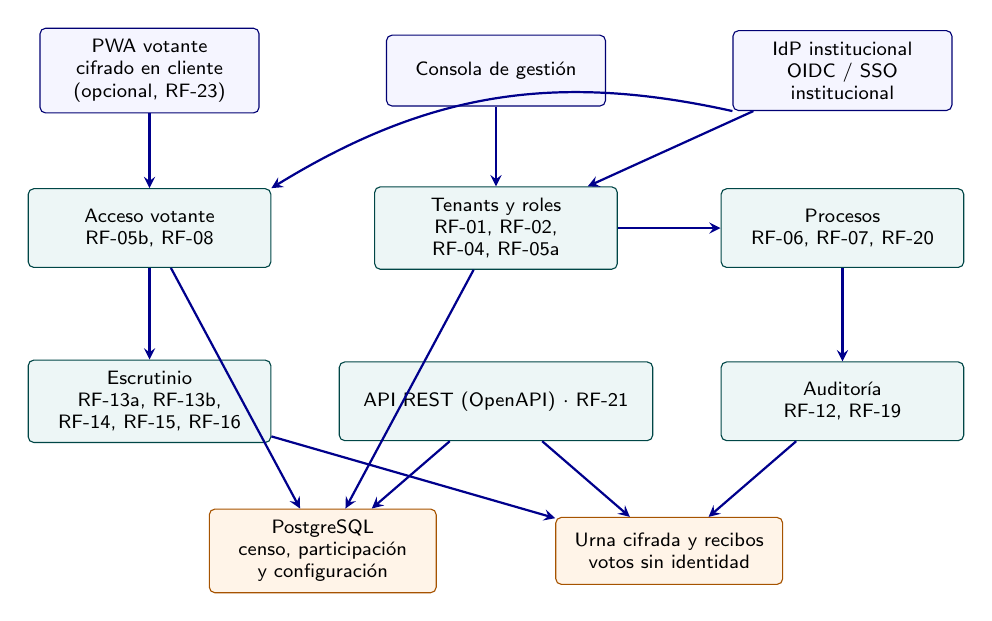
\begin{tikzpicture}[
  font=\sffamily\scriptsize,
  box/.style={draw=blue!45!black, rounded corners=2pt, fill=blue!4,
    align=center, minimum height=0.9cm, text width=2.5cm, inner sep=4pt},
  mod/.style={draw=teal!55!black, rounded corners=2pt, fill=teal!7,
    align=center, minimum height=1cm, text width=2.8cm, inner sep=4pt},
  store/.style={draw=orange!65!black, rounded corners=2pt, fill=orange!9,
    align=center, minimum height=0.85cm, text width=2.6cm, inner sep=4pt},
  link/.style={->,>=stealth, thick, draw=blue!55!black},
  optional/.style={->,>=stealth, dashed, thick, draw=gray!75}
]
\node[box] (pwa) at (0,0) {PWA votante\\cifrado en cliente (opcional, RF-23)};
\node[box] (gest) at (4.4,0) {Consola de gestión};
\node[box] (idp) at (8.8,0) {IdP institucional\\OIDC / SSO institucional};

\node[mod] (access) at (0,-2.0) {Acceso votante\\RF-05b, RF-08};
\node[mod] (tenant) at (4.4,-2.0) {Tenants y roles\\RF-01, RF-02, RF-04, RF-05a};
\node[mod] (election) at (8.8,-2.0) {Procesos\\RF-06, RF-07, RF-20};

\node[mod] (ballot) at (0,-4.2) {Escrutinio\\RF-13a, RF-13b, RF-14, RF-15, RF-16};
\node[mod,text width=3.7cm] (api) at (4.4,-4.2) {API REST (OpenAPI) $\cdot$ RF-21};
\node[mod] (audit) at (8.8,-4.2) {Auditoría\\RF-12, RF-19};

\node[store] (db) at (2.2,-6.1) {PostgreSQL\\censo, participación y configuración};
\node[store] (urn) at (6.6,-6.1) {Urna cifrada y recibos\\votos sin identidad};

\draw[link] (pwa) -- (access);
\draw[link] (gest) -- (tenant);
\draw[link] (idp) -- (tenant);
\draw[link] (idp.south west) to[bend right=22] (access.north east);
\draw[link] (access) -- (ballot);
\draw[link] (tenant) -- (election);
\draw[link] (election) -- (audit);
\draw[link] (ballot) -- (urn);
\draw[link] (access) -- (db);
\draw[link] (tenant) -- (db);
\draw[link] (api) -- (db);
\draw[link] (api) -- (urn);
\draw[link] (audit) -- (urn);
\end{tikzpicture}
}
  \caption{Arquitectura objetivo de la plataforma SaaS de votación (no representa el despliegue implementado).}
  \label{fig:arquitectura-componentes}
\end{figure}

\section{Secuencia de emisión y verificación del voto}
\label{sec:secuencia-voto}

La figura~\ref{fig:secuencia-emision-voto} representa el flujo lógico de
emisión, pero conserva nombres conceptuales de la especificación. En la
implementación, voter-access consume el token y ballot-box guarda el voto, el
hash del recibo y el evento en una transacción. El registro de participación
solo conserva el día; la urna no almacena identidad ni marca temporal por voto.
El recibo acredita presencia (RF-10), mientras que la cadena se verifica por
separado (RF-12).

\begin{figure}[p]
  \centering
  \resizebox{0.94\textwidth}{!}{% Secuencia vectorial en TikZ. Emisión (1--8) y verificación (9--11).
\begin{tikzpicture}[x=1.1cm,y=0.75cm,font=\sffamily\scriptsize,
  life/.style={draw=gray!65,dashed},
  msg/.style={-{Stealth},draw=gray!70,thick},
  ret/.style={-{Stealth},draw=gray!70,dashed,thick},
  participant/.style={draw=teal!55!black,fill=teal!6,rounded corners=2pt,align=center,
    text width=1.55cm,minimum height=.74cm,inner sep=2pt}]
\node[participant] (pwa) at (0,0) {PWA\\votante};
\node[participant] (access) at (2,0) {Voter-access\\API};
\node[participant] (receipt) at (4,0) {Ballot-box\\API};
\node[participant] (census) at (6,0) {Voter-access\\DB};
\node[participant] (ballot) at (8,0) {pg-ballot\\votos};
\node[participant] (audit) at (10,0) {pg-ballot\\eventos};
\foreach \x in {0,2,4,6,8,10} \draw[life] (\x,-0.55)--(\x,-10.15);

\draw[rounded corners,draw=gray!55] (-0.7,-0.9) rectangle (10.7,-7.05);
\node[anchor=west,fill=white] at (-0.6,-0.82) {Emisión (1--8)};
\draw[rounded corners,draw=gray!55] (-0.7,-7.35) rectangle (10.7,-10.4);
\node[anchor=west,fill=white] at (-0.6,-7.27) {Verificación del recibo (9--11)};

\draw[msg] (0,-1.4)--node[above]{1 enlace + método}(2,-1.4);
\draw[ret] (2,-2.1)--node[above]{2 token de un uso}(0,-2.1);
\draw[msg] (0,-2.9)--node[above]{3 voto + token}(4,-2.9);
\draw[msg] (4,-3.7)--node[above]{4 valida y consume}(2,-3.7);
\draw[ret] (2,-4.4)--node[above]{5 resultado}(4,-4.4);
\draw[msg] (2,-5.1)--node[above]{participación: día}(6,-5.1);
\draw[msg] (4,-5.8)--node[above]{6 voto + hash recibo}(8,-5.8);
\draw[msg] (8,-6.4)--node[above]{7 evento encadenado}(10,-6.4);
\draw[ret] (4,-6.8)--node[above]{8 recibo}(0,-6.8);

\draw[msg] (0,-7.95)--node[above]{9 verificar}(4,-7.95);
\draw[msg] (4,-8.75)--node[above]{10 buscar recibo}(8,-8.75);
\draw[ret] (4,-9.55)--node[above]{11 consta}(0,-9.55);

\node[draw=gray!55,rounded corners=2pt,align=left,text width=10.4cm,inner sep=4pt]
  at (5,-11.55) {El método configurado es código por correo o cuenta institucional. Ballot-box valida y consume el token mediante voter-access; el registro de participación conserva solo el día. Voto, hash del recibo y evento se guardan en una transacción en pg-ballot. No se cifra el voto en cliente. RF-10 comprueba presencia del recibo; RF-12 verifica la cadena por separado. Flecha continua: llamada; discontinua: respuesta.};
\end{tikzpicture}
}
\caption{Flujo lógico de emisión del voto y verificación de presencia del recibo.}
  \label{fig:secuencia-emision-voto}
\end{figure}

\section{Actividad de escrutinio y verificación del resultado}
\label{sec:actividad-escrutinio}

La figura~\ref{fig:actividad-escrutinio} modela el cierre de la urna, la
comprobación de integridad, el cálculo del escrutinio y la publicación o
retención del resultado según la verificación de la cadena de auditoría
(RF-13).

\begin{figure}[htbp]
  \centering
  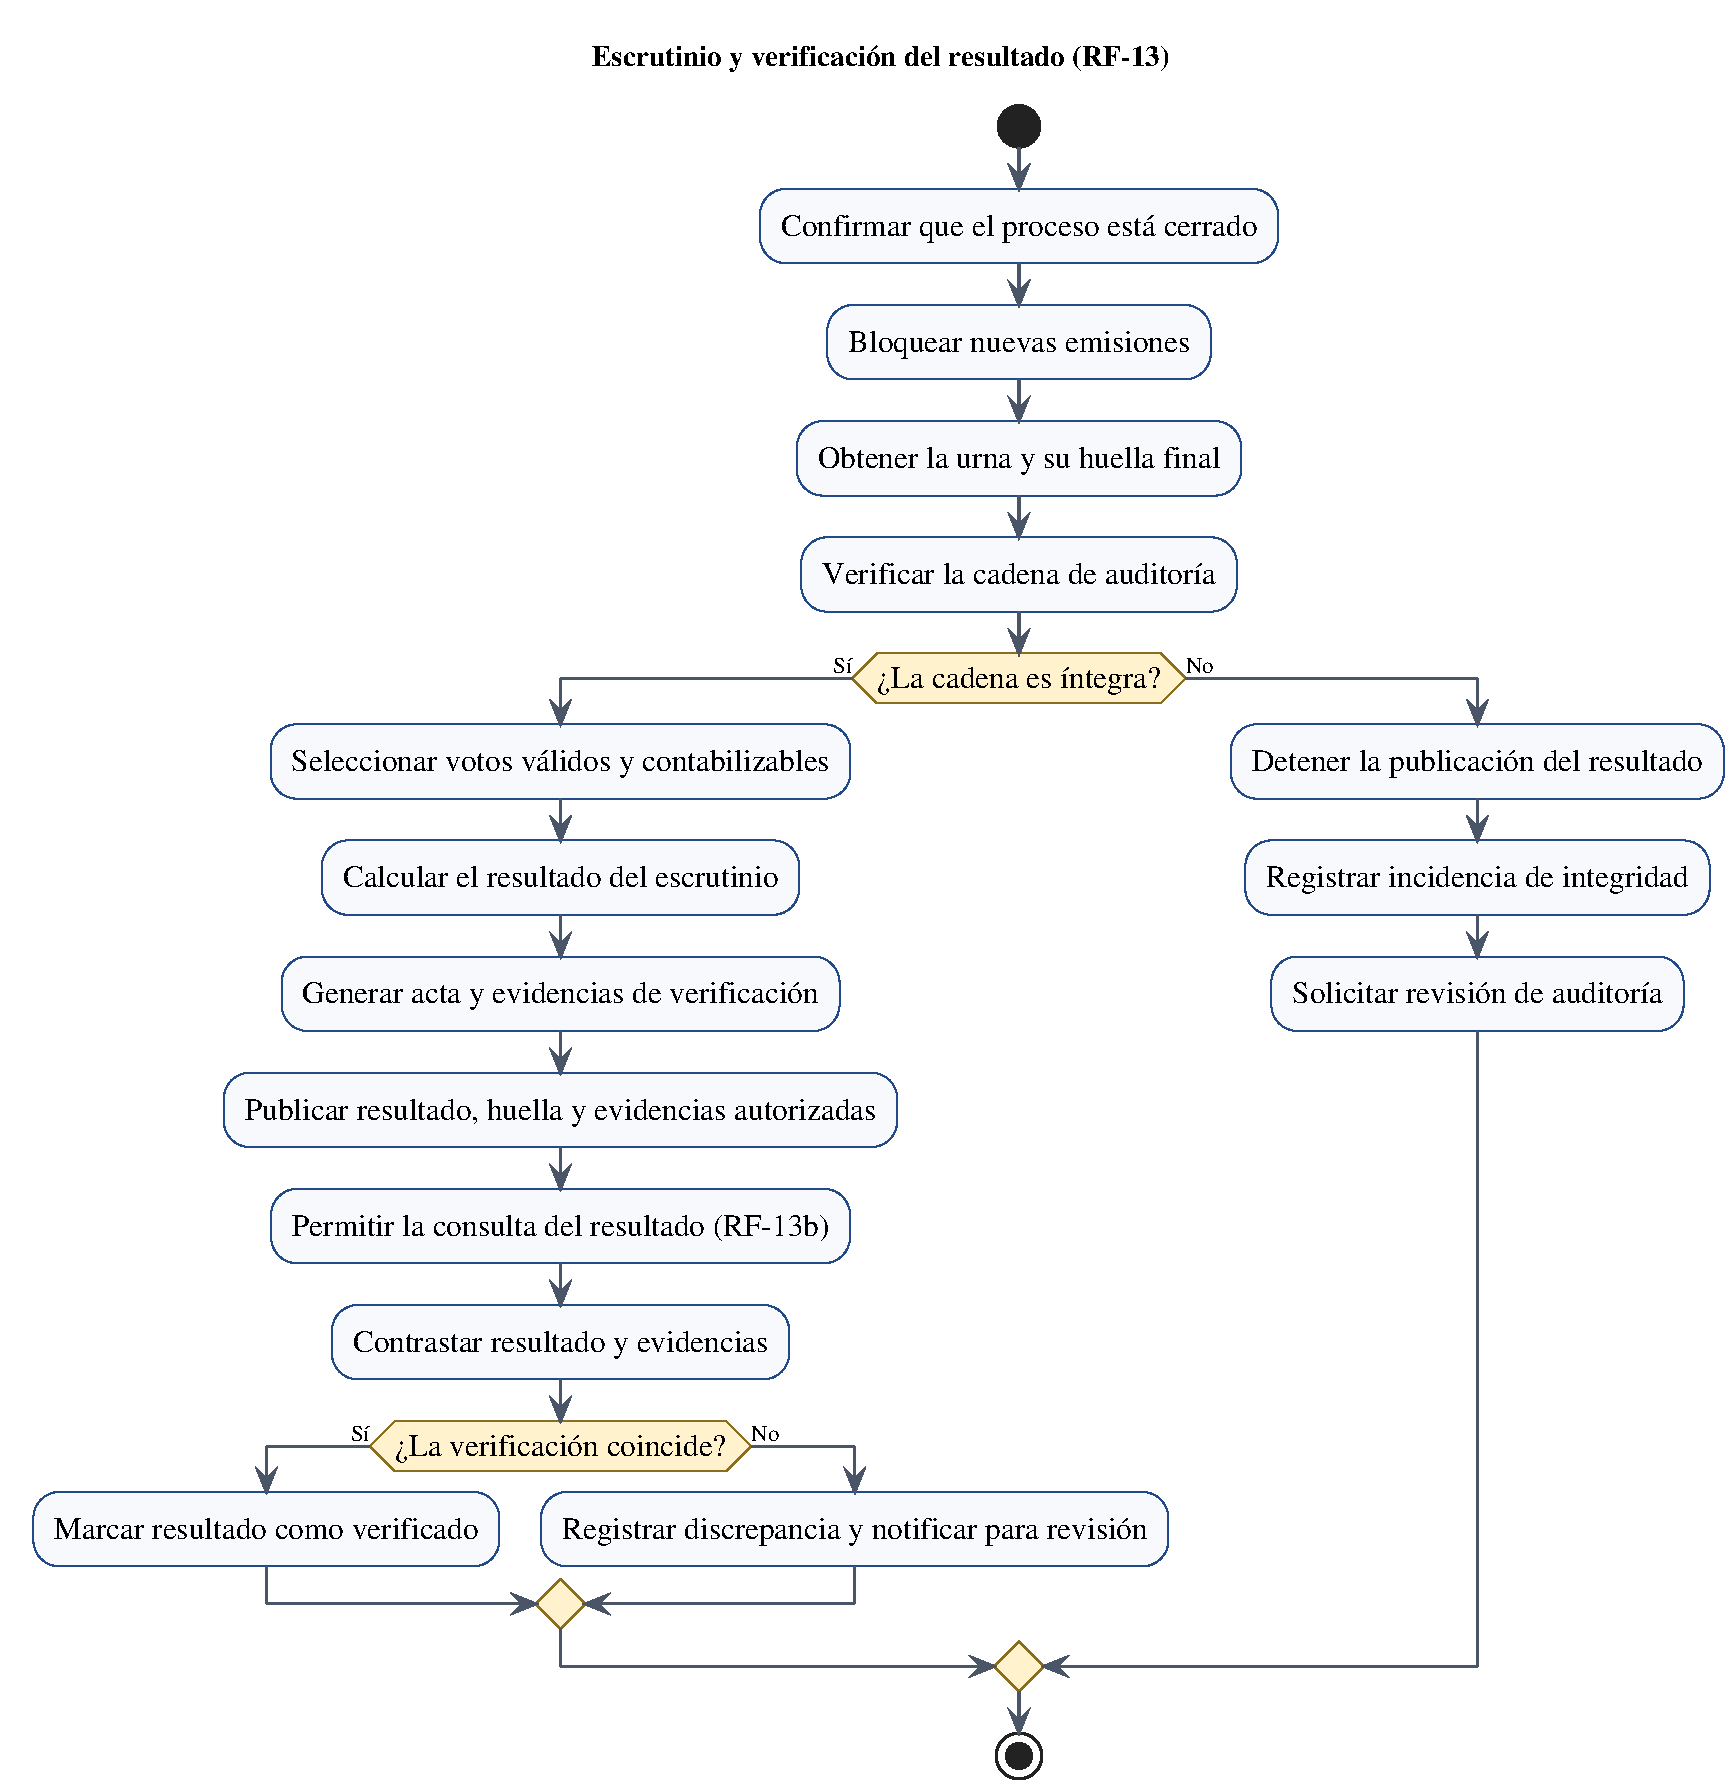
\includegraphics[width=0.90\textwidth,height=0.68\textheight,keepaspectratio]{Figuras/diagramas/escrutinio_verificacion_actividad.pdf}
  \caption{Actividad de escrutinio y verificación del resultado (RF-13).}
  \label{fig:actividad-escrutinio}
\end{figure}

\section{Separación de información y confianza}
\label{sec:separacion-informacion}

El modelo conceptual distingue los datos de identidad y censo, los registros
de participación, la urna, los recibos, los eventos de auditoría y los
resultados. Esta separación persigue que el sistema pueda controlar la
unicidad y mostrar la participación sin conservar una relación directa entre
la persona y su opción elegida. La integridad del registro se apoya en huellas
encadenadas; el diseño técnico deberá especificar su generación, protección,
publicación y verificación.

\section{Criterios de calidad y validación}
\label{sec:validacion-calidad}

La validación deberá relacionar cada requisito con evidencias concretas:
pruebas de accesibilidad con teclado y lector de pantalla, pruebas de
usabilidad, concurrencia y carga, revisión de aislamiento multi-tenant,
comprobación de registros y evaluación de los flujos de protección de datos.
Los criterios cuantitativos se tratarán como objetivos propuestos hasta su
aprobación por las partes interesadas.

% Capítulos de apoyo elaborados a partir de los requisitos del proyecto.
\chapter{Especificación detallada de requisitos}
\label{cap:especificacion-detallada}

Este capítulo desarrolla los flujos de los casos de uso y los requisitos
de información y calidad recogidos en la especificación de origen. Se
conservan los códigos para mantener la trazabilidad entre documentos.

\textbf{Nota de alcance.} Las referencias a re-votación o sustitución (RF-11,
estados “Sustituido” y “re-votación permitida”) proceden de la especificación
v1.0 y no están implementadas en el MVP (D-03). El estado “Sustituido” se
conserva en el modelo como referencia de diseño para RF-11 (P9), pero no es
operativo: la urna registra un único voto aceptado por token de emisión y no
genera ese estado.

\section{Casos de uso}
\label{sec:casos-uso-detallados}

\subsection{RF-01: Gestionar organizaciones}

\textbf{Objetivos asociados:} OBJ-1\par
\textbf{Requisitos asociados:} RI-1\par
\textbf{Descripción:} El sistema deberá comportarse como se describe a continuación cuando un Superadministrador (ACT-1) da de alta una organización.\par
\textbf{Precondición:} El usuario está autenticado (RF-04) como Superadministrador.\par
\textbf{Flujo normal:}
\begin{enumerate}
\item[1] El Superadministrador solicita dar de alta una organización
\item[2] El Sistema solicita el nombre, identificador y administrador inicial de la organización.
\item[3] El Superadministrador introduce los datos solicitados.
\item[4] El Sistema comprueba que el identificador no está en uso.
\item[5] El Sistema crea la organización con su espacio de datos aislado y asigna el rol de Administrador de organización al administrador inicial.
\end{enumerate}
\textbf{Postcondición:} La organización existe con su espacio de datos aislado y el administrador inicial tiene asignado el rol de Administrador de organización.\par
\textbf{Excepciones y alternativas:}
\begin{itemize}
\item 4: Si el identificador ya está en uso, el Sistema informa de la situación y solicita introducir otro identificador.
\end{itemize}
\textbf{Comentarios:} Ninguno\par

\subsection{RF-02: Gestionar roles y permisos}

\textbf{Objetivos asociados:} OBJ-1\par
\textbf{Requisitos asociados:} RI-2\par
\textbf{Descripción:} El sistema deberá comportarse como se describe a continuación cuando un Administrador de organización (ACT-2) asigna o cambia el rol de un usuario de su organización (el Superadministrador (ACT-1) puede hacerlo en cualquier organización).\par
\textbf{Precondición:} El usuario está autenticado y el usuario destino pertenece a la organización.\par
\textbf{Flujo normal:}
\begin{enumerate}
\item[1] El Administrador solicita gestionar usuarios y roles
\item[2] El Sistema muestra los usuarios de la organización con su rol
\item[3] El Administrador selecciona un usuario o solicita crear uno nuevo
\item[4] El Sistema muestra los roles asignables
\item[5] El Administrador selecciona el rol
\item[6] El Sistema guarda el rol y aplica sus permisos desde la siguiente acción del usuario
\end{enumerate}
\textbf{Postcondición:} El usuario tiene el nuevo rol y sus permisos efectivos.\par
\textbf{Excepciones y alternativas:}
\begin{itemize}
\item 5: Si se intenta dejar la organización sin Administrador, el Sistema lo impide e informa
\item 5: Si el actor no puede asignar ese rol, el Sistema deniega la operación
\end{itemize}
\textbf{Comentarios:} Prioridad M. Se asume que solo un Superadministrador puede asignar el rol de Superadministrador.\par

\subsection{RF-03: Gestionar censo}

\textbf{Objetivos asociados:} OBJ-2\par
\textbf{Requisitos asociados:} RI-3, RNF-4\par
\textbf{Descripción:} El sistema deberá comportarse como se describe a continuación cuando un Administrador da de alta, importa o modifica votantes del censo.\par
\textbf{Precondición:} El Gestor de censo está autenticado.\par
\textbf{Flujo normal:}
\begin{enumerate}
\item[1] El Gestor solicita gestionar el censo
\item[2] El Sistema muestra los censos existentes
\item[3] El Gestor elige la acción
\item[]\textit{Si elige alta manual:}
\item[3.1] El Sistema solicita nombre, email o teléfono
\item[3.2] El Gestor introduce los datos
\item[]\textit{Si elige importar CSV:}
\item[3.1] El Sistema solicita el fichero CSV
\item[3.2] El Gestor selecciona el fichero
\item[3.3] El Sistema valida el fichero y muestra un resumen (altas, duplicados, errores)
\item[3.4] El Gestor confirma la importación
\item[4] El Sistema detecta duplicados y no los da de alta
\item[5] El Sistema guarda los cambios e informa del resultado
\end{enumerate}
\textbf{Postcondición:} El censo está actualizado y sin duplicados.\par
\textbf{Excepciones y alternativas:}
\begin{itemize}
\item 3.3: Si el fichero no es válido, el Sistema informa de las líneas erróneas y permite descartarlas o cancelar
\item 4: Si hay duplicados, el Sistema los omite e informa de cuáles
\item 5: Si el censo pertenece a un proceso abierto, el Sistema rechaza altas y bajas e informa
\end{itemize}
\textbf{Comentarios:} Prioridad M. Se asume que el censo queda congelado mientras el proceso está abierto.\par

\subsection{RF-04: Autenticar usuario de gestión}

\textbf{Objetivos asociados:} OBJ-1\par
\textbf{Requisitos asociados:} RI-2\par
\textbf{Descripción:} El sistema deberá comportarse como se describe a continuación cuando un Superadministrador, Administrador, Gestor de censo o Auditor desea iniciar sesión.\par
\textbf{Precondición:} La cuenta existe y está activa.\par
\textbf{Flujo normal:}
\begin{enumerate}
\item[1] El Usuario solicita iniciar sesión
\item[2] El Sistema solicita usuario y contraseña
\item[3] El Usuario introduce sus credenciales
\item[4] El Sistema valida las credenciales
\item[5] El Sistema solicita el segundo factor
\item[6] El Usuario introduce el segundo factor
\item[7] El Sistema valida el segundo factor
\item[8] El Sistema inicia la sesión y muestra la pantalla de inicio de su rol
\end{enumerate}
\textbf{Postcondición:} Sesión iniciada con el rol y la organización correspondientes.\par
\textbf{Excepciones y alternativas:}
\begin{itemize}
\item 4: Si las credenciales son incorrectas, el Sistema informa del error y permite reintentar.
\item 7: Si el código del segundo factor es incorrecto o ha caducado, el Sistema informa del error y permite reintentar o solicitar un nuevo código.
\end{itemize}
\textbf{Comentarios:} Prioridad M. La autenticación se realiza mediante el mecanismo configurado para la plataforma. Como opción de diseño, podrá integrarse un proveedor de identidad compatible con OIDC/SSO (RF-05); no se exige una cuenta institucional. El segundo factor podrá realizarse mediante un código enviado al correo electrónico del usuario.\par

\subsection{RF-05: Iniciar sesión (RF-05a gestión y RF-05b votante)}

\textbf{Objetivos asociados:} OBJ-1, OBJ-3\par
\textbf{Requisitos asociados:} RI-2, RI-3\par
\textbf{Descripción:} El sistema deberá permitir que los perfiles de gestión (RF-05a) y los votantes (RF-05b) inicien sesión mediante el mecanismo de autenticación habilitado para la plataforma o el proceso. La integración con un proveedor de identidad (ACT-6), por ejemplo mediante OIDC/SSO, es una opción de diseño.\par
\textbf{Precondición:} La cuenta está activa o, en el caso del votante, pertenece al censo del proceso. Si se usa un proveedor externo, este está configurado y disponible.\par
\textbf{Flujo normal:}
\begin{enumerate}
\item[1] El usuario solicita iniciar sesión y elige uno de los mecanismos habilitados
\item[2] El Sistema solicita las credenciales o inicia el flujo del proveedor de identidad, si está configurado
\item[3] El usuario se autentica con el mecanismo seleccionado
\item[4] El Sistema valida la respuesta y comprueba la cuenta, el rol y, cuando corresponda, la pertenencia al censo
\item[5] El Sistema inicia la sesión o concede el acceso al proceso
\end{enumerate}
\textbf{Postcondición:} Sesión iniciada con el rol y el ámbito de organización o proceso correspondientes.\par
\textbf{Excepciones y alternativas:}
\begin{itemize}
\item 3: Si el usuario cancela o no se autentica, el Sistema vuelve a la pantalla de inicio
\item 2--4: Si el proveedor no responde, las credenciales son incorrectas o la respuesta no es válida, el Sistema informa y permite reintentar o usar otro mecanismo habilitado
\item 4: Si la cuenta no tiene un rol autorizado o el votante no figura en el censo, el Sistema deniega el acceso e informa
\end{itemize}
\textbf{Comentarios:} Prioridad Should. El requisito describe el inicio de sesión de forma independiente del proveedor y del protocolo. OIDC/SSO es una alternativa de diseño que deberá concretarse si se adopta; no implica SSO institucional obligatorio.\par

\subsection{RF-06: Crear y configurar proceso de votación}

\textbf{Objetivos asociados:} OBJ-2\par
\textbf{Requisitos asociados:} RI-4, RI-5, RNF-4\par
\textbf{Descripción:} El sistema deberá comportarse como se describe a continuación cuando un Administrador de organización (ACT-2) crea y configura un proceso de votación, incluyendo la definición del tipo de voto y de la papeleta.\par
\textbf{Precondición:} El Administrador está autenticado y existe un censo (RF-03).\par
\textbf{Flujo normal:}
\begin{enumerate}
\item[1] El Administrador solicita crear un proceso
\item[2] El Sistema solicita título y descripción
\item[3] El Administrador introduce el título y la descripción.
\item[4] El Sistema solicita el calendario (apertura y cierre)
\item[5] El Administrador introduce fechas y horas
\item[6] El Sistema solicita el censo participante.
\item[7] El Administrador selecciona el censo participante.
\item[8] El Sistema solicita definir la papeleta.
\item[9] El Sistema muestra los tipos de voto disponibles: opción única y sí/no/abstención.
\item[10] El Administrador selecciona el tipo de voto.
\item[11] El Administrador introduce las opciones y decide si habilita el voto en blanco.
\end{enumerate}
\textbf{Postcondición:} El proceso de votación existe en estado Borrador con su papeleta definida.\par
\textbf{Excepciones y alternativas:}
\begin{itemize}
\item 12: Si existen datos incompletos o incoherentes en el proceso o en la papeleta, el Sistema informa del error y permite corregir los datos sin guardar.
\end{itemize}
\textbf{Comentarios:} Prioridad M. Incluye la definición del tipo de voto y de la papeleta.\par

\subsection{RF-07: Gestionar ciclo de vida del proceso}

\textbf{Objetivos asociados:} OBJ-2\par
\textbf{Requisitos asociados:} RI-4, RI-9\par
\textbf{Descripción:} El sistema deberá comportarse como se describe a continuación cuando un Administrador de organización (ACT-2) programa y archiva un proceso, y el Sistema lo abre y lo cierra automáticamente en las fechas fijadas.\par
\textbf{Precondición:} El proceso existe y el Administrador está autenticado.\par
\textbf{Flujo normal:}
\begin{enumerate}
\item[1] El Administrador solicita programar el proceso
\item[2] El Sistema valida que el proceso está completo.
\item[3] El Sistema cambia el proceso a Programado
\item[4] Al llegar la fecha de apertura, el Sistema cambia el proceso a Abierto y habilita el acceso de los votantes (RF-08)
\item[5] Al llegar la fecha de cierre, el Sistema cambia el proceso a Cerrado y deja de aceptar votos
\item[6] El Sistema publica la huella final de la urna (RF-12), inicia el escrutinio (RF-13) y, al terminar, cambia el proceso a Escrutado
\item[7] El Administrador solicita archivar el proceso
\item[8] El Sistema cambia el proceso a Archivado
\end{enumerate}
\textbf{Postcondición:} Estado del proceso actualizado y registrado (RF-19).\par
\textbf{Excepciones y alternativas:}
\begin{itemize}
\item 2: Si el proceso está incompleto, el Sistema informa y no lo programa.
\end{itemize}
\textbf{Comentarios:} Prioridad M. Lo amplían RF-13 (escrutinio al cerrar) y RF-17 (avisos). No se permite abrir ni cerrar un proceso manualmente de forma anticipada; la apertura y el cierre se realizan automáticamente en las fechas configuradas.\par

\subsection{RF-08: Acceder como votante}

\textbf{Objetivos asociados:} OBJ-3\par
\textbf{Requisitos asociados:} RI-3, RI-12, RNF-1, RNF-2, RNF-3, RNF-5, RNF-9\par
\textbf{Descripción:} El sistema deberá comportarse como se describe a continuación cuando un Votante (ACT-4) accede a la papeleta de un proceso abierto; el código lo envía el Servicio de notificaciones (ACT-7).\par
\textbf{Precondición:} El proceso está Abierto, el votante está en el censo y ha recibido su enlace personal (RF-17).\par
\textbf{Flujo normal:}
\begin{enumerate}
\item[1] El Votante abre su enlace personal
\item[2] El Sistema valida el enlace y que el proceso está abierto
\item[3] El Sistema solicita la verificación adicional del proceso
\item[]\textit{Si es un código OTP:}
\item[3.1] El Sistema envía el código por email
\item[3.2] El Votante introduce el código
\item[3.3] El Sistema valida el código
\item[4] El Sistema concede acceso a la papeleta
\end{enumerate}
\textbf{Postcondición:} El votante está identificado para ese proceso.\par
\textbf{Excepciones y alternativas:}
\begin{itemize}
\item 2: Si el enlace no es válido o ha caducado, el Sistema informa y no concede acceso
\item 2: Si el proceso no está abierto, el Sistema informa de su estado y calendario
\item 3.3: Si el código es incorrecto o ha caducado, el Sistema permite reintentar o reenviarlo.
\end{itemize}
\textbf{Comentarios:} Prioridad M. La verificación adicional configurada (por ejemplo, OTP o autenticación federada) evita que un enlace reenviado permita votar a otra persona. La federación de identidad es una opción de diseño, no un requisito institucional.\par

\subsection{RF-09: Emitir voto}

\textbf{Objetivos asociados:} OBJ-3\par
\textbf{Requisitos asociados:} RI-5, RI-6, RI-7, RNF-1, RNF-2, RNF-3, RNF-5, RNF-7, RNF-9\par
\textbf{Descripción:} El sistema deberá comportarse como se describe a continuación cuando un Votante (ACT-4) emite su voto en un proceso abierto.\par
\textbf{Precondición:} El votante ha accedido (RF-08) y no tiene un voto contabilizado, o el proceso permite re-votar (RF-11).\par
\textbf{Flujo normal:}
\begin{enumerate}
\item[1] El Sistema muestra la papeleta.
\item[2] El Votante selecciona sus opciones
\item[3] El Sistema valida la selección según el tipo de papeleta
\item[4] El Sistema muestra un resumen y pide confirmación
\item[5] El Votante confirma
\item[6] El Sistema comprueba que no hay ya un voto contabilizado del votante
\item[7] El Sistema registra el voto en la urna.
\item[8] El Sistema marca al votante como «ha votado»
\item[9] El Sistema confirma la emisión y ofrece el recibo (RF-10)
\end{enumerate}
\textbf{Postcondición:} El voto está en la urna y el votante figura como votante.\par
\textbf{Excepciones y alternativas:}
\begin{itemize}
\item 3: Si la selección no es válida, el Sistema informa y no avanza
\item 6: Si el votante ya votó y no se permite re-votar, el Sistema informa y no registra nada
\item 7: Si el proceso se cierra mientras vota o falla el registro, el Sistema informa y no queda ningún voto parcial ni duplicado
\end{itemize}
\textbf{Comentarios:} Prioridad M. El voto se registra en la urna y el votante queda marcado como «ha votado». Como máximo se contabiliza un voto por votante.\par

\subsection{RF-10: Obtener y verificar recibo del voto}

\textbf{Objetivos asociados:} OBJ-3, OBJ-4\par
\textbf{Requisitos asociados:} RI-6, RI-8, RNF-1, RNF-2, RNF-3, RNF-6\par
\textbf{Descripción:} El sistema deberá comportarse como se describe a continuación cuando un Votante (ACT-4) quiere comprobar que su voto consta en la urna.\par
\textbf{Precondición:} El votante ha emitido un voto (RF-09).\par
\textbf{Flujo normal:}
\begin{enumerate}
\item[1] El Sistema genera un recibo del voto.
\item[2] El Sistema entrega el recibo al votante
\item[3] El Votante solicita verificar su recibo
\item[4] El Sistema busca el recibo en la urna publicada
\item[5] El Sistema informa de que el voto consta en la urna
\end{enumerate}
\textbf{Postcondición:} Ninguna.\par
\textbf{Excepciones y alternativas:}
\begin{itemize}
\item 4: Si el recibo no se encuentra, el Sistema informa de que el voto no consta
\end{itemize}
\textbf{Comentarios:} Prioridad M. Amplía RF-09. Si el votante vuelve a votar (RF-11), el recibo anterior se marca como sustituido.\par

\subsection{RF-11: Re-votar}

\textbf{Estado en el MVP:} No implementado. D-03 excluye RF-11 del MVP; la exclusión fue confirmada por el tutor el 30/10/2026 mediante correo electrónico, y el caso de uso permanece como trabajo futuro (P9). Se conserva aquí por trazabilidad con la especificación v1.0.\par

\textbf{Objetivos asociados:} OBJ-3\par
\textbf{Requisitos asociados:} RI-6, RI-7, RI-8, RNF-1, RNF-2, RNF-7, RNF-9\par
\textbf{Descripción:} El sistema deberá comportarse como se describe a continuación cuando un Votante (ACT-4) cambia su voto antes del cierre.\par
\textbf{Precondición:} El proceso está Abierto, permite re-votación y el votante ya ha votado y ha accedido (RF-08).\par
\textbf{Flujo normal:}
\begin{enumerate}
\item[1] El Votante solicita cambiar su voto
\item[2] El Sistema informa de que el nuevo voto sustituirá al anterior
\item[3] El Votante confirma
\item[4] El Votante emite el nuevo voto (RF-09)
\item[5] El Sistema registra el nuevo voto y marca el anterior como sustituido sin borrarlo
\item[6] El Sistema entrega el nuevo recibo
\end{enumerate}
\textbf{Postcondición:} Solo cuenta el último voto del votante.\par
\textbf{Excepciones y alternativas:}
\begin{itemize}
\item 3: Si la votante cancela, su voto anterior sigue siendo válido
\item 5: Si el proceso se cierra antes de registrar el nuevo voto, el anterior sigue siendo válido
\end{itemize}
\textbf{Comentarios:} Prioridad W (fuera de esta versión; era C en la especificación v1.0). Amplía RF-15. La re-votación mitiga la coacción: el votante puede cambiar su voto hasta el cierre.\par

\subsection{RF-12: Publicar y verificar registro de auditoría}

\textbf{Objetivos asociados:} OBJ-4\par
\textbf{Requisitos asociados:} RI-9\par
\textbf{Descripción:} El sistema deberá comportarse como se describe a continuación cuando un Auditor (ACT-3) consulta y verifica el registro de la urna, o un Votante (ACT-4) consulta la huella publicada.\par
\textbf{Precondición:} Existe un proceso con eventos en la urna.\par
\textbf{Flujo normal:}
\begin{enumerate}
\item[1] El Auditor solicita ver el registro de auditoría de un proceso
\item[2] El Sistema muestra los eventos de la urna (apertura, votos recibidos sin identidad, sustituciones, cierre) con su huella
\item[3] El Auditor solicita verificar la integridad
\item[4] El Sistema comprueba la integridad del registro.
\item[5] El Sistema informa del resultado de la verificación
\item[]\textit{Si el proceso está cerrado:}
\item[6] El Sistema muestra la huella final publicada, que cualquier Votante puede consultar
\end{enumerate}
\textbf{Postcondición:} Ninguna.\par
\textbf{Excepciones y alternativas:}
\begin{itemize}
\item 2: Si el proceso no tiene eventos, el Sistema informa
\item 5: Si la cadena está rota, el Sistema alerta al Auditor y al Administrador y marca una incidencia de integridad
\end{itemize}
\textbf{Comentarios:} Prioridad S.\par

\subsection{RF-13: Escrutar y verificar resultado}

\textbf{Objetivos asociados:} OBJ-4\par
\textbf{Requisitos asociados:} RI-4, RI-6, RI-10, RNF-6\par
\textbf{Descripción:} El sistema deberá comportarse como se describe a continuación cuando un proceso se cierra y el Sistema lanza automáticamente el escrutinio; después, un Auditor (ACT-3) o un Votante (ACT-4) verifica el resultado.\par
\textbf{Precondición:} El proceso está Cerrado.\par
\textbf{Flujo normal:}
\begin{enumerate}
\item[1] El Sistema lanza el escrutinio al cerrarse el proceso
\item[2] El Sistema obtiene los votos contabilizables (el último de cada votante).
\item[3] El Sistema cuenta los votos por opción.
\item[4] El Sistema calcula la participación.
\item[5] El Sistema guarda el resultado y publica su huella.
\item[6] El Auditor o el Votante solicita verificar el resultado
\item[7] El Sistema muestra los datos públicos necesarios para recalcularlo
\item[8] El Sistema informa de si el resultado coincide
\end{enumerate}
\textbf{Postcondición:} Proceso en estado Escrutado con resultado y huella publicados.\par
\textbf{Excepciones y alternativas:}
\begin{itemize}
\item 5: Si falla el recuento, el Sistema no publica nada, avisa al Administrador y permite reintentar.
\item 8: Si no coincide, el Sistema alerta de una incidencia
\end{itemize}
\textbf{Comentarios:} Prioridad M. Amplía RF-07. Queda por decidir qué significa «público»: cualquier persona o solo los participantes del proceso.\par

\subsection{RF-14: Consultar panel de participación}

\textbf{Objetivos asociados:} OBJ-4\par
\textbf{Requisitos asociados:} RI-3, RI-7\par
\textbf{Descripción:} El sistema deberá comportarse como se describe a continuación cuando un Administrador de organización (ACT-2) consulta la participación de un proceso.\par
\textbf{Precondición:} El Administrador está autenticado.\par
\textbf{Flujo normal:}
\begin{enumerate}
\item[1] El Administrador solicita el panel de participación
\item[2] El Sistema muestra el número de votantes del censo, los votos emitidos y el porcentaje de participación.
\item[3] El Sistema actualiza el panel mientras el proceso está abierto.
\end{enumerate}
\textbf{Postcondición:} Ninguna.\par
\textbf{Excepciones y alternativas:}
\begin{itemize}
\item 2: Si el proceso aún no está abierto, el Sistema muestra solo el censo
\item 2: Si el proceso está cerrado, muestra la participación final
\end{itemize}
\textbf{Comentarios:} Prioridad M. Ninguna vista muestra el recuento por opción antes del cierre.\par

\subsection{RF-15: Consultar y exportar resultados}

\textbf{Objetivos asociados:} OBJ-4\par
\textbf{Requisitos asociados:} RI-10\par
\textbf{Descripción:} El sistema deberá comportarse como se describe a continuación cuando un Administrador de organización (ACT-2), o un Votante (ACT-4) si el proceso lo permite, consulta y exporta los resultados.\par
\textbf{Precondición:} El proceso está Escrutado.\par
\textbf{Flujo normal:}
\begin{enumerate}
\item[1] El usuario solicita ver los resultados
\item[2] El Sistema comprueba que el usuario puede verlos
\item[3] El Sistema muestra los resultados con gráficos y participación.
\item[4] El usuario solicita exportarlos
\item[5] El Sistema genera el fichero en formato CSV y lo entrega.
\end{enumerate}
\textbf{Postcondición:} Ninguna.\par
\textbf{Excepciones y alternativas:}
\begin{itemize}
\item 2: Si el proceso no está escrutado, el Sistema informa de que aún no hay resultados
\item 2: Si el usuario no tiene permiso, el Sistema deniega el acceso
\end{itemize}
\textbf{Comentarios:} Prioridad M. Los resultados pueden ser consultados por el Administrador de organización y por los votantes cuando el proceso lo permita. La exportación de resultados se realiza únicamente en formato CSV.\par

\subsection{RF-16: Generar acta de resultados en PDF}

\textbf{Objetivos asociados:} OBJ-4\par
\textbf{Requisitos asociados:} RI-10\par
\textbf{Descripción:} El sistema deberá comportarse como se describe a continuación cuando un Administrador de organización (ACT-2) genera el acta de un proceso.\par
\textbf{Precondición:} El proceso está Escrutado y el Administrador está autenticado.\par
\textbf{Flujo normal:}
\begin{enumerate}
\item[1] El Administrador solicita el acta
\item[2] El Sistema compone el acta (proceso, calendario, censo, participación, resultado y huellas)
\item[3] El Sistema genera el PDF y lo ofrece para descarga
\item[4] El Administrador lo descarga
\end{enumerate}
\textbf{Postcondición:} Acta disponible en PDF con huella.\par
\textbf{Excepciones y alternativas:}
\begin{itemize}
\item 1: Si el proceso no está escrutado, el Sistema informa de que el acta no está disponible
\item 3: Si falla la generación, el Sistema informa y permite reintentar
\end{itemize}
\textbf{Comentarios:} Prioridad S. Amplía RF-15. El contenido del acta debe validarse con las exigencias de cada organización.\par

\subsection{RF-17: Enviar notificaciones}

\textbf{Objetivos asociados:} OBJ-3\par
\textbf{Requisitos asociados:} RI-11, RI-12\par
\textbf{Descripción:} El sistema deberá comportarse como se describe a continuación cuando se programa, abre o cierra un proceso y el Sistema avisa a los votantes mediante el Servicio de notificaciones (ACT-7). El Administrador de organización (ACT-2) configura las plantillas y los canales.\par
\textbf{Precondición:} El proceso está programado y el Administrador ha configurado plantillas y canales.\par
\textbf{Flujo normal:}
\begin{enumerate}
\item[1] El Sistema inicia el envío de invitaciones al programarse el proceso
\item[2] El Sistema genera el enlace personal de cada votante (RF-08) y compone el mensaje en su idioma
\item[3] El Sistema entrega los mensajes al Servicio de notificaciones
\item[4] El Servicio de notificaciones informa del resultado de entrega
\item[5] El Sistema registra el estado de cada envío
\item[6] En las fechas configuradas, el Sistema envía recordatorios a quien aún no ha votado
\item[7] Al cierre, el Sistema envía el aviso de cierre
\end{enumerate}
\textbf{Postcondición:} Votantes avisados y estado de envío registrado.\par
\textbf{Excepciones y alternativas:}
\begin{itemize}
\item 4: Si una entrega falla, el Sistema reintenta y la marca; el Administrador puede consultar los fallos
\item 2: Si un votante no tiene dato de contacto para el canal, el Sistema lo omite y lo lista.
\end{itemize}
\textbf{Comentarios:} Prioridad M. Amplía RF-08.\par

\subsection{RF-18: Gestionar privacidad de datos (RGPD)}

\textbf{Objetivos asociados:} OBJ-1\par
\textbf{Requisitos asociados:} RI-2, RI-3\par
\textbf{Descripción:} El sistema deberá comportarse como se describe a continuación cuando un Administrador de organización (ACT-2) exporta o borra los datos personales de un interesado a petición de este.\par
\textbf{Precondición:} El Administrador está autenticado.\par
\textbf{Flujo normal:}
\begin{enumerate}
\item[1] El Administrador solicita la gestión de privacidad
\item[]\textit{Si exporta datos de un interesado:}
\item[2.1] El Administrador identifica al interesado.
\item[2.2] El Sistema compila sus datos personales y los exporta en formato legible por máquina.
\item[]\textit{Si borra datos de un interesado:}
\item[3.1] El Administrador identifica al interesado y confirma la solicitud de borrado.
\item[3.2] El Sistema borra o anonimiza sus datos personales.
\end{enumerate}
\textbf{Postcondición:} Los datos del interesado han sido exportados o borrados, según la solicitud.\par
\textbf{Excepciones y alternativas:}
\begin{itemize}
\item 3.2: Si el interesado ya votó, el Sistema anonimiza sus datos personales y conserva el voto y el registro de auditoría.
\end{itemize}
\textbf{Comentarios:} Prioridad S. El voto no es exportable por interesado porque no está vinculado a su identidad. Si el votante ya ha votado, se anonimizan sus datos personales y se conserva el voto.\par

\subsection{RF-19: Consultar trazabilidad de acciones}

\textbf{Objetivos asociados:} OBJ-4\par
\textbf{Requisitos asociados:} RI-13\par
\textbf{Descripción:} El sistema deberá comportarse como se describe a continuación cuando un Auditor (ACT-3) o un Administrador de organización (ACT-2) consulta las acciones administrativas registradas.\par
\textbf{Precondición:} El usuario está autenticado. El Sistema registra automáticamente cada acción administrativa.\par
\textbf{Flujo normal:}
\begin{enumerate}
\item[1] El usuario solicita la trazabilidad
\item[2] El Sistema solicita filtros (fechas, usuario, tipo de acción, proceso)
\item[3] El usuario los introduce
\item[4] El Sistema muestra las acciones: quién, qué, sobre qué objeto y cuándo
\end{enumerate}
\textbf{Postcondición:} Ninguna.\par
\textbf{Excepciones y alternativas:}
\begin{itemize}
\item 4: Si no hay resultados, el Sistema informa
\end{itemize}
\textbf{Comentarios:} Prioridad S. El registro lo hace el Sistema en cada caso de uso de administración y no se puede editar. El Administrador solo ve las acciones de su organización.\par

\section{Requisitos de información}
\label{sec:datos-detallados}

\subsection{RI-1: Información sobre organizaciones}

\textbf{Objetivos asociados:} OBJ-1\par
\textbf{Requisitos asociados:} RF-01\par
\textbf{Descripción:} El sistema deberá almacenar la información correspondiente a las organizaciones (tenants) que utilizan la plataforma.\par
\textbf{Datos específicos:} Identificador de organización: 20 caracteres alfanuméricos (único) Nombre visible: 100 caracteres Estado: Activa o Suspendida Fecha de alta: dd/mm/aaaa hh:mm\par
\textbf{Comentarios:} Los datos de cada organización están aislados lógicamente de los de las demás (arquitectura multi-tenant).\par

\subsection{RI-2: Información sobre usuarios y roles}

\textbf{Objetivos asociados:} OBJ-1\par
\textbf{Requisitos asociados:} RF-01, RF-02, RF-04, RF-05\par
\textbf{Descripción:} El sistema deberá almacenar la información correspondiente a los usuarios de gestión de la plataforma y a su rol.\par
\textbf{Datos específicos:} Identificador de usuario: entero positivo Organización: identificador de organización (RI-1) Nombre y apellidos: 60 caracteres Correo electrónico: 100 caracteres (único por organización) Teléfono: 15 dígitos (opcional) Rol: Superadministrador, Administrador o Auditor Contraseña: se almacena solo su huella (hash) Segundo factor activado: Sí o No Estado de la cuenta: Activa, Bloqueada o Inactiva Fecha del último acceso: dd/mm/aaaa hh:mm\par
\textbf{Comentarios:} Los votantes no son usuarios de gestión: se almacenan en el censo (RI-3). Se asume que un usuario pertenece a una única organización, salvo el Superadministrador, que pertenece a la plataforma.\par

\subsection{RI-3: Información sobre censo}

\textbf{Objetivos asociados:} OBJ-2\par
\textbf{Requisitos asociados:} RF-03, RF-05, RF-08, RF-14, RF-18\par
\textbf{Descripción:} El sistema deberá almacenar la información correspondiente a los votantes de cada organización.\par
\textbf{Datos específicos:} Identificador de votante: entero positivo Organización: identificador de organización (RI-1) Nombre y apellidos: 60 caracteres Correo electrónico: 100 caracteres Teléfono: 15 dígitos (opcional) Identificador externo: 50 caracteres (opcional, solo si el mecanismo de autenticación seleccionado lo requiere)\par
\textbf{Comentarios:} El control de duplicados se hace mediante los datos definidos por la organización, como el correo electrónico; un identificador externo solo se conserva si resulta necesario para el mecanismo configurado.\par

\subsection{RI-4: Información sobre procesos de votación}

\textbf{Objetivos asociados:} OBJ-2\par
\textbf{Requisitos asociados:} RF-06, RF-07, RF-08, RF-09, RF-12, RF-13, RF-14.\par
\textbf{Descripción:} El sistema deberá almacenar la información correspondiente a los procesos de votación y a su configuración.\par
\textbf{Datos específicos:} Identificador del proceso: entero positivo Organización: identificador de organización (RI-1) Título: 150 caracteres Descripción: 1000 caracteres Fecha de apertura: dd/mm/aaaa hh:mm Fecha de cierre: dd/mm/aaaa hh:mm (posterior a la de apertura) Estado: Borrador, Programado, Abierto, Cerrado, Escrutado o Archivado Re-votación permitida: Sí o No\par
\textbf{Comentarios:} El estado del proceso determina qué operaciones están permitidas (RF-08).\par

\subsection{RI-5: Información sobre papeletas}

\textbf{Objetivos asociados:} OBJ-2\par
\textbf{Requisitos asociados:} RF-06, RF-09, RF-10, RF-11\par
\textbf{Descripción:} El sistema deberá almacenar la información correspondiente a la papeleta de cada proceso, incluidas sus traducciones.\par
\textbf{Datos específicos:} Tipo de voto: Opción única o Sí/No/Abstención Pregunta: 300 caracteres Opciones (lista): texto de la opción (200 caracteres) y orden (entero positivo) Voto en blanco habilitado: Sí o No\par
\textbf{Comentarios:} Si falta una traducción, se muestra el texto en el idioma por defecto del proceso.\par

\subsection{RI-6: Información sobre votos (urna)}

\textbf{Objetivos asociados:} OBJ-3, OBJ-4\par
\textbf{Requisitos asociados:} RF-09, RF-10, RF-11, RF-13\par
\textbf{Descripción:} El sistema deberá almacenar los votos emitidos en cada proceso, sin ninguna relación con la identidad del votante.\par
\textbf{Datos específicos:} Identificador del voto: 36 caracteres (identificador aleatorio) Proceso: identificador del proceso (RI-4) Contenido del voto: opción elegida Fecha y hora de recepción: dd/mm/aaaa hh:mm:ss Canal: En línea Estado: Contabilizable o Sustituido\par
\textbf{Comentarios:} El voto no contiene ningún identificador ni dato de contacto del votante. Cuando un votante vuelve a votar (RF-11), el voto anterior pasa a Sustituido, sin borrarse. Solo se escrutan los votos Contabilizables. En el MVP el estado Sustituido no se genera (D-03): se conserva como referencia de diseño para RF-11 (P9), y activarlo requiere implementar la sustitución y validarla con pruebas de concurrencia y unicidad.\par

\subsection{RI-7: Información sobre participación}

\textbf{Objetivos asociados:} OBJ-3\par
\textbf{Requisitos asociados:} RF-08, RF-09, RF-11, RF-14\par
\textbf{Descripción:} El sistema deberá almacenar qué votantes han participado en cada proceso, sin indicar qué han votado.\par
\textbf{Datos específicos:} Proceso: identificador del proceso (RI-4) Votante: identificador de votante (RI-3) Ha votado: Sí o No Fecha y hora del último voto: dd/mm/aaaa hh:mm Canal del voto: En línea\par
\textbf{Comentarios:} Este registro se guarda separado de la urna (RI-6) y no enlaza con ningún voto concreto. Permite calcular la participación y evitar votos duplicados (RF-08/09).\par

\subsection{RI-8: Información sobre recibos de verificación}

\textbf{Objetivos asociados:} OBJ-3, OBJ-4\par
\textbf{Requisitos asociados:} RF-10, RF-11\par
\textbf{Descripción:} El sistema deberá almacenar la información correspondiente a los recibos que permiten al votante verificar su voto.\par
\textbf{Datos específicos:} Código del recibo: 64 caracteres hexadecimales Proceso: identificador del proceso (RI-4) Fecha y hora de emisión: dd/mm/aaaa hh:mm:ss Estado: Vigente o Sustituido\par
\textbf{Comentarios:} El recibo permite comprobar que el voto consta en la urna sin revelar su contenido. El recibo no se asocia a la identidad del votante.\par

\subsection{RI-9: Información sobre registro de auditoría de la urna}

\textbf{Objetivos asociados:} OBJ-4\par
\textbf{Requisitos asociados:} RF-07, RF-12\par
\textbf{Descripción:} El sistema deberá almacenar el registro encadenado de los eventos de la urna de cada proceso.\par
\textbf{Datos específicos:} Número de secuencia: entero positivo Proceso: identificador del proceso (RI-4) Tipo de evento: Apertura, Voto recibido, Voto sustituido, Cierre o Publicación de huella Fecha y hora: dd/mm/aaaa hh:mm:ss Huella del evento: 64 caracteres hexadecimales Huella del evento anterior: 64 caracteres hexadecimales Huella final publicada: 64 caracteres hexadecimales (solo tras el cierre)\par
\textbf{Comentarios:} Cada evento incluye la huella del anterior, de modo que cualquier alteración rompe la cadena y se detecta al verificarla (RF-12). Los eventos de voto no incluyen datos del votante.\par

\subsection{RI-10: Información sobre resultados y actas}

\textbf{Objetivos asociados:} OBJ-4\par
\textbf{Requisitos asociados:} RF-13, RF-15, RF-16\par
\textbf{Descripción:} El sistema deberá almacenar el resultado del escrutinio de cada proceso y el acta generada.\par
\textbf{Datos específicos:} Proceso: identificador del proceso (RI-4) Fecha del escrutinio: dd/mm/aaaa hh:mm Resultado por opción (lista): opción, votos (entero positivo) y porcentaje (número real con 2 cifras decimales) Votos en blanco: entero positivo Participación: número real (con 2 cifras decimales, en porcentaje) Huella del resultado: 64 caracteres hexadecimales Acta: fichero PDF Fecha de generación del acta: dd/mm/aaaa hh:mm\par
\textbf{Comentarios:} El resultado solo existe cuando el proceso está escrutado.\par

\subsection{RI-11: Información sobre notificaciones}

\textbf{Objetivos asociados:} OBJ-3\par
\textbf{Requisitos asociados:} RF-17\par
\textbf{Descripción:} El sistema deberá almacenar la información correspondiente a las notificaciones enviadas a los votantes y su estado de entrega.\par
\textbf{Datos específicos:} Identificador de notificación: entero positivo Proceso: identificador del proceso (RI-4) Votante: identificador de votante (RI-3) Tipo: Invitación, Recordatorio, Cierre Canal: Correo electrónico Plantilla: texto de hasta 1000 caracteres Fecha y hora de envío: dd/mm/aaaa hh:mm Estado: Pendiente, Entregada o Fallida Número de reintentos: entero de 1 cifra\par
\textbf{Comentarios:} Las plantillas y los canales los configura el Administrador de organización. Las notificaciones fallidas se pueden consultar (RF-17).\par

\subsection{RI-12: Información sobre acceso de votantes}

\textbf{Objetivos asociados:} OBJ-3\par
\textbf{Requisitos asociados:} RF-08, RF-17\par
\textbf{Descripción:} El sistema deberá almacenar la información necesaria para que cada votante acceda a la papeleta de un proceso abierto.\par
\textbf{Datos específicos:} Proceso: identificador del proceso (RI-4) Votante: identificador de votante (RI-3) Enlace personal: 64 caracteres (identificador aleatorio) Fecha de caducidad del enlace: dd/mm/aaaa hh:mm Código de verificación (OTP): 6 dígitos, se almacena solo su huella Fecha de caducidad del código: dd/mm/aaaa hh:mm Intentos fallidos: entero de 1 cifra Bloqueado hasta: dd/mm/aaaa hh:mm\par
\textbf{Comentarios:} El enlace personal identifica a un único votante en un único proceso. Tras varios intentos fallidos, el acceso se bloquea temporalmente.\par

\subsection{RI-13: Información sobre trazabilidad de acciones administrativas}

\textbf{Objetivos asociados:} OBJ-4\par
\textbf{Requisitos asociados:} RF-19\par
\textbf{Descripción:} El sistema deberá almacenar el registro de las acciones administrativas realizadas en la plataforma.\par
\textbf{Datos específicos:} Identificador de acción: entero positivo Fecha y hora: dd/mm/aaaa hh:mm:ss Usuario: identificador de usuario (RI-2) Organización: identificador de organización (RI-1) Tipo de acción: 50 caracteres Objeto afectado: 100 caracteres Detalle: 500 caracteres\par
\textbf{Comentarios:} El registro lo crea el Sistema automáticamente y no se puede modificar ni borrar. Es distinto del registro de auditoría de la urna (RI-10), que solo recoge eventos de la votación.\par

\section{Requisitos no funcionales}
\label{sec:rnf-detallados}

Los requisitos RNF-8 y RNF-10 se aplican de forma transversal a todos los
casos de uso (RF-01 a RF-19) y a todas las pantallas del sistema. No se
asocian a un caso de uso concreto.

\subsection{RNF-1: Accesibilidad WCAG 2.2 AA}

\textbf{Objetivos asociados:} OBJ-3\par
\textbf{Requisitos asociados:} RF-08, RF-09, RF-10, RF-11\par
\textbf{Descripción:} Las pantallas del votante deberán seguir el nivel AA de las pautas WCAG 2.2. Criterio de aceptación: cero incumplimientos críticos ni serios en las pantallas evaluadas, más revisión manual con teclado y lector de pantalla sin bloqueos en el flujo de acceso, voto y recibo.\par
\textbf{Comentarios:} Verificación: auditoría automática (por ejemplo, axe o Lighthouse) y revisión manual con teclado y lector de pantalla (H1a). La auditoría automática no certifica conformidad WCAG. Un incumplimiento serio puntual se documentará como incidencia y se decidirá si se corrige antes del cierre; el criterio no se relaja a priori. Criterio validado por el tutor. Sustituye al antiguo RF-18.\par

\subsection{RNF-2: Diseño adaptable y navegadores}

\textbf{Objetivos asociados:} OBJ-3\par
\textbf{Requisitos asociados:} RF-08, RF-09, RF-10, RF-11\par
\textbf{Descripción:} La interfaz deberá ser usable desde pantallas de 360 px de ancho, sin desplazamiento horizontal, y funcionar en las dos últimas versiones de Chrome, Firefox, Safari y Edge.\par
\textbf{Comentarios:} Verificación: pruebas en móvil, tableta y ordenador con cada navegador. Los valores (360 px, dos versiones) son propuestos. Sustituye al antiguo RF-18.\par

\subsection{RNF-3: Facilidad de uso del votante}

\textbf{Objetivos asociados:} OBJ-3\par
\textbf{Requisitos asociados:} RF-08, RF-09, RF-10, RF-11\par
\textbf{Descripción:} Las cinco personas no técnicas y sin formación previa que participen en la prueba deberán completar sin ayuda el acceso, el voto y la obtención del recibo en 3 minutos o menos.\par
\textbf{Comentarios:} Verificación: test de usabilidad con cinco personas no técnicas (H1b). Criterio del protocolo validado por el tutor. Con $n = 5$ no hay inferencia estadística: los resultados son evidencia descriptiva limitada al prototipo, la configuración y la población evaluados.\par

\subsection{RNF-4: Facilidad de uso del administrador}

\textbf{Objetivos asociados:} OBJ-1, OBJ-2\par
\textbf{Requisitos asociados:} RF-03, RF-06, RF-07\par
\textbf{Descripción:} Al menos 4 de 5 administradores de organización sin formación previa deberán crear, configurar y programar un proceso de opción única en 10 minutos o menos y sin ayuda. «Sin ayuda» significa sin intervención del moderador ni de otras personas; consultar la documentación de la herramienta sí está permitido.\par
\textbf{Comentarios:} Verificación: test de usabilidad con cinco personas con perfil de administrador. El valor de 10 minutos es propuesto. Con $n = 5$ no hay inferencia estadística: los resultados serán evidencia descriptiva limitada al prototipo, la configuración y la población evaluados. No hay hipótesis asociada en la sección~\ref{sec:plan-evaluacion}. La sesión del 03/11/2026 no cumplió las condiciones del criterio (población sin formación previa y tiempos medidos), por lo que RNF-4 se presenta como no demostrado en el capítulo de evaluación.\par

\subsection{RNF-5: Idiomas de la interfaz}

\textbf{Objetivos asociados:} OBJ-3\par
\textbf{Requisitos asociados:} RF-08, RF-09\par
\textbf{Descripción:} La interfaz deberá estar disponible en español e inglés, con todos los textos en ficheros de recursos, de modo que añadir un idioma no exija cambiar código. Cambiar de idioma no debe hacer perder los datos introducidos.\par
\textbf{Comentarios:} Verificación: revisión de código y prueba de cambio de idioma durante el flujo de voto.\par

\subsection{RNF-6: Claridad de la verificación del voto}

\textbf{Objetivos asociados:} OBJ-3, OBJ-4\par
\textbf{Requisitos asociados:} RF-10, RF-13\par
\textbf{Descripción:} La pantalla de verificación del recibo y del resultado deberá explicarse en lenguaje no técnico, sin términos criptográficos en el mensaje principal, y al menos 4 de las 5 personas no técnicas que participen en la prueba deberán interpretar correctamente si su voto consta en la urna.\par
\textbf{Comentarios:} Verificación: test con cinco personas no técnicas (H1b). Responde al objetivo de mejorar la usabilidad de la verificación para votantes no técnicos. Criterio del protocolo validado por el tutor. Con $n = 5$ no hay inferencia estadística: los resultados son evidencia descriptiva limitada al prototipo, la configuración y la población evaluados.\par

\subsection{RNF-7: Prevención de errores al votar}

\textbf{Objetivos asociados:} OBJ-3\par
\textbf{Requisitos asociados:} RF-09, RF-11.\par
\textbf{Descripción:} Antes de registrar un voto, el sistema deberá mostrar siempre un resumen de la selección y pedir confirmación explícita, y avisar de cualquier selección no válida antes de avanzar de pantalla.\par
\textbf{Comentarios:} Verificación: prueba funcional con todos los tipos de papeleta (RF-09), incluidas selecciones no válidas.\par

\subsection{RNF-8: Mensajes de error y realimentación}

\textbf{Objetivos asociados:} OBJ-1, OBJ-2, OBJ-3, OBJ-4\par
\textbf{Requisitos asociados:} Todos los requisitos funcionales (RF-01 a RF-19)\par
\textbf{Descripción:} Todo error mostrado al usuario deberá indicar con lenguaje claro qué ha ocurrido y cómo corregirlo, sin códigos técnicos. Toda acción que tarde más de 1 segundo deberá mostrar un indicador de progreso y toda acción completada deberá mostrar una confirmación visible.\par
\textbf{Comentarios:} Verificación: revisión de los mensajes de las excepciones de los casos de uso y prueba cronometrada de las acciones lentas. El valor de 1 segundo es propuesto.\par

\subsection{RNF-9: Orientación del votante durante el voto}

\textbf{Objetivos asociados:} OBJ-3\par
\textbf{Requisitos asociados:} RF-08, RF-09, RF-11.\par
\textbf{Descripción:} En cada paso del voto (acceso, selección, confirmación y recibo), el votante deberá ver en qué paso está y cuántos quedan, y en todo momento el estado del proceso y su hora de cierre.\par
\textbf{Comentarios:} Verificación: revisión de las pantallas del flujo de voto y test de usabilidad (RNF-3).\par

\subsection{RNF-10: Consistencia de la interfaz}

\textbf{Objetivos asociados:} OBJ-1, OBJ-2, OBJ-3, OBJ-4\par
\textbf{Requisitos asociados:} RF-01 a RF-19\par
\textbf{Descripción:} La interfaz deberá usar la misma terminología, la misma ubicación de los elementos de navegación y los mismos componentes en todas las pantallas, sin problemas graves de consistencia en una revisión heurística.\par
\textbf{Comentarios:} Verificación: revisión heurística (heurísticas de Nielsen) por al menos 2 evaluadores, sin problemas de gravedad alta. Los valores son propuestos.\par

\subsection{RNF-11: Secreto del voto}

\textbf{Objetivos asociados:} OBJ-3, OBJ-4\par
\textbf{Requisitos asociados:} RF-09, RF-10, RF-11, RF-13\par
\textbf{Descripción:} Ninguna tabla enlaza voto e identidad. La urna (RI-6) y la participación (RI-7) están separadas.\par
\textbf{Comentarios:} Verificación: revisión del modelo de datos y prueba de no correlación.\par

\subsection{RNF-12: Unicidad}

\textbf{Objetivos asociados:} OBJ-3\par
\textbf{Requisitos asociados:} RF-09, RF-11\par
\textbf{Descripción:} El sistema deberá garantizar que solo un voto sea contabilizado por votante, incluso cuando se produzcan envíos simultáneos.\par
\textbf{Comentarios:} Verificación: prueba de envíos concurrentes del mismo votante para comprobar que únicamente un voto queda en estado Contabilizable.\par

\subsection{RNF-13: Integridad y trazabilidad}

\textbf{Objetivos asociados:} OBJ-4\par
\textbf{Requisitos asociados:} RF-12, RF-19\par
\textbf{Descripción:} El registro usa hash encadenado y cualquier alteración se detecta. Toda acción administrativa queda registrada y no es editable.\par
\textbf{Comentarios:} Verificación: prueba de alteración del registro y auditoría.\par

\subsection{RNF-14: Seguridad de acceso}

\textbf{Objetivos asociados:} OBJ-1, OBJ-3\par
\textbf{Requisitos asociados:} RF-04, RF-08\par
\textbf{Descripción:} Contraseñas con hash y sal. Bloqueo tras 5 intentos fallidos. Segundo factor. HTTPS. Sesión con caducidad.\par
\textbf{Comentarios:} Verificación: pruebas de seguridad. Valores propuestos.\par

\subsection{RNF-15: Aislamiento entre organizaciones}

\textbf{Objetivos asociados:} OBJ-1\par
\textbf{Requisitos asociados:} RF-01\par
\textbf{Descripción:} Ningún usuario accede a datos de otra organización, comprobado con pruebas.\par
\textbf{Comentarios:} Verificación: pruebas de acceso cruzado entre tenants.\par

\subsection{RNF-16: Protección de datos (RGPD)}

\textbf{Objetivos asociados:} OBJ-1\par
\textbf{Requisitos asociados:} RF-18\par
\textbf{Descripción:} El sistema deberá limitar la recogida de datos personales a los estrictamente necesarios para la prestación del servicio y deberá permitir su eliminación cuando corresponda conforme a la normativa aplicable.\par
\textbf{Comentarios:} Verificación: revisión del modelo de datos y prueba del flujo de eliminación de datos personales.\par

\subsection{RNF-17: Rendimiento}

\textbf{Objetivos asociados:} OBJ-3\par
\textbf{Requisitos asociados:} RF-09, RF-13\par
\textbf{Descripción:} El sistema deberá soportar al menos 500 votantes simultáneos durante la emisión de votos y deberá responder en menos de 2 segundos en al menos el 95 \% de las peticiones realizadas durante dicha carga.\par
\textbf{Comentarios:} Verificación: prueba de carga con al menos 500 usuarios simultáneos y medición del tiempo de respuesta. Los valores establecidos son propuestos y deberán validarse con el cliente.\par

\subsection{RNF-18: Portabilidad (PWA instalable)}

\textbf{Objetivos asociados:} OBJ-3\par
\textbf{Requisitos asociados:} RF-08, RF-09\par
\textbf{Descripción:} La aplicación deberá ser instalable como PWA en dispositivos móviles.\par
\textbf{Comentarios:} Prioridad C. Verificación: instalación en Android e iOS.\par


\chapter{Mapeo de los requisitos no funcionales con ISO/IEC 25010:2023}
\label{cap:rnf-iso25010}

La norma ISO/IEC 25010:2023 define un modelo de calidad de producto con nueve
características y subcaracterísticas que sirven de referencia para especificar y
evaluar la calidad del software \citep{isoiec25010_2023}. La tabla~\ref{tab:rnf-iso25010}
relaciona los RNF de la plataforma con las características que describen mejor
su intención. El mapeo es una clasificación razonada, no una certificación de
conformidad con la norma.

RNF-8 y RNF-10 son transversales a todos los casos de uso (RF-01 a RF-19) y a
todas las pantallas; no se asocian a un caso de uso concreto. Esta
transversalidad se aplica en la especificación y en la verificación del
producto.

\small
\begin{longtable}{|p{0.07\textwidth}|p{0.20\textwidth}|p{0.21\textwidth}|p{0.34\textwidth}|p{0.12\textwidth}|}
\caption{Correspondencia de los RNF con ISO/IEC 25010:2023.}\label{tab:rnf-iso25010}\\
\hline
\textbf{RNF} & \textbf{Característica} & \textbf{Subcaracterística} & \textbf{Justificación} & \textbf{Prioridad (MoSCoW)} \\
\hline
\endfirsthead
\hline
\textbf{RNF} & \textbf{Característica} & \textbf{Subcaracterística} & \textbf{Justificación} & \textbf{Prioridad (MoSCoW)} \\
\hline
\endhead
\hline
\multicolumn{5}{r}{Continúa en la página siguiente.}\\
\endfoot
\hline
\endlastfoot
RNF-1 & Capacidad de interacción & Inclusivity; User assistance & WCAG 2.2 AA, teclado y lector de pantalla facilitan el uso a personas con distintas capacidades. & Por validar \\
\hline
RNF-2 & Capacidad de interacción; Flexibilidad; Compatibilidad & Operability; Adaptability; Interoperability & El diseño para 360 px exige adaptación; el soporte de varios navegadores requiere interoperabilidad y operación coherente. & Por validar \\
\hline
RNF-3 & Capacidad de interacción & Learnability; Operability & Mide si una persona sin formación aprende y completa el flujo de voto con eficacia. & Por validar \\
\hline
RNF-4 & Capacidad de interacción & Learnability; Operability & Mide si un administrador aprende a configurar un proceso sin asistencia. & Por validar \\
\hline
RNF-5 & Capacidad de interacción & Inclusivity & La disponibilidad en español e inglés contempla diferencias lingüísticas entre usuarios. & Por validar \\
\hline
RNF-6 & Capacidad de interacción & Self-descriptiveness & El lenguaje no técnico permite entender, sin ayuda externa, qué indica la verificación. & Por validar \\
\hline
RNF-7 & Capacidad de interacción & User error protection & El resumen, la confirmación y la detección temprana de selecciones inválidas previenen errores de voto. & Por validar \\
\hline
RNF-8 & Capacidad de interacción & Self-descriptiveness; User assistance & Los mensajes claros, el progreso y la confirmación explican el estado y la siguiente acción; el RNF no especifica tolerancia técnica a fallos. & Por validar \\
\hline
RNF-9 & Capacidad de interacción & Operability; Self-descriptiveness & El indicador de pasos y el estado del proceso orientan al votante durante la operación. & Por validar \\
\hline
RNF-10 & Capacidad de interacción & Operability & La terminología y los controles consistentes hacen predecible la navegación entre pantallas. & Por validar \\
\hline
RNF-11 & Seguridad & Confidentiality & Separar la urna de la participación evita que usuarios no autorizados relacionen identidad y voto. & Por validar \\
\hline
RNF-12 & Seguridad; Fiabilidad & Integrity; Faultlessness & La unicidad impide que un envío concurrente altere el estado correcto de contabilización. & Por validar \\
\hline
RNF-13 & Seguridad & Integrity; Accountability; Non-repudiation & El encadenamiento detecta alteraciones y los registros inmutables permiten atribuir y probar acciones. & Por validar \\
\hline
RNF-14 & Seguridad & Authenticity; Resistance; Confidentiality & La autenticación y los controles frente a intentos indebidos protegen las sesiones y la información. & Por validar \\
\hline
RNF-15 & Seguridad & Confidentiality & El aislamiento entre tenants restringe el acceso a datos a los usuarios de cada organización. & Por validar \\
\hline
RNF-16 & Seguridad & Confidentiality & La minimización y eliminación limitan la exposición de datos personales; el RGPD es una restricción normativa, no una subcaracterística de ISO 25010. & Por validar \\
\hline
RNF-17 & Eficiencia de desempeño & Time behaviour; Capacity & El umbral de respuesta mide el comportamiento temporal y los 500 usuarios simultáneos expresan capacidad. & Por validar \\
\hline
RNF-18 & Flexibilidad & Installability; Adaptability & La instalación como PWA en móviles requiere instalabilidad y adaptación a distintas plataformas. & Could \\
\hline
\end{longtable}
\normalsize

\noindent\footnotesize Las prioridades RNF no consignadas en la especificación
se muestran como «Por validar»; RNF-18 conserva la prioridad Could allí
indicada.\normalsize

Los nombres de subcaracterísticas se conservan en inglés para mantener la
terminología de la edición 2023. En particular, el requisito RNF-2 también se
relaciona con Compatibilidad porque especifica funcionamiento en distintos
navegadores; y RNF-8 no se asigna a Fiabilidad, pues describe realimentación de
interfaz, pero no continuidad del servicio ante fallos.

\chapter{Diagrama de casos de uso}
\label{cap:refactorizacion-diagrama}

Para que los nombres y las relaciones se lean con claridad, los casos de uso
se presentan en dos diagramas PlantUML independientes: gestión y
configuración en la figura~\ref{fig:casos-uso-gestion}; participación y
verificación en la figura~\ref{fig:casos-uso-votacion}. Las fuentes editables
se guardan en \texttt{Figuras/diagramas/}.

\begin{figure}[p]
  \centering
  \resizebox{0.94\textwidth}{!}{% Diagrama vectorial simplificado para lectura en la memoria.
\begin{tikzpicture}[font=\sffamily\scriptsize,
  actor/.style={draw=blue!55!black,fill=blue!4,rounded corners=2pt,align=center,text width=2.0cm,minimum height=.62cm,inner sep=3pt},
  uc/.style={draw=gray!65!black,fill=blue!3,ellipse,align=center,text width=3.0cm,minimum height=.72cm,inner sep=2pt},
  rel/.style={draw=gray!70,thin},
  gen/.style={draw=gray!70,thin,-{Triangle[open]}}]
\node[font=\bfseries\small] at (4,5.8) {Casos de uso: gestión y configuración};
\draw[rounded corners,draw=gray!55] (0.5,-5.5) rectangle (7.6,5.35);
\node[fill=white,font=\bfseries] at (4,5.35) {Plataforma SaaS (Gestión)};

\node[uc] (rf01) at (2.5,4.55) {RF-01\\Organizaciones};
\node[uc] (rf02) at (2.5,3.55) {RF-02\\Roles y permisos};
\node[uc] (rf03) at (2.5,2.55) {RF-03\\Gestionar censo};
\node[uc] (rf04) at (2.5,1.55) {RF-04\\Autenticar gestión};
\node[uc] (rf05) at (2.5,.55) {RF-05a\\Iniciar sesión gestión};
\node[uc] (rf06) at (2.5,-.45) {RF-06\\Configurar proceso};
\node[uc] (rf07) at (2.5,-1.45) {RF-07\\Ciclo de vida};
\node[uc] (rf14) at (2.5,-2.45) {RF-14\\Consultar participación};
\node[uc] (rf16) at (2.5,-3.45) {RF-16\\Generar acta PDF};
\node[uc] (rf17) at (2.5,-4.45) {RF-17\\Enviar notificaciones};
\node[uc] (rf18) at (5.8,3.55) {RF-18\\Privacidad RGPD};
\node[uc] (rf19) at (5.8,1.55) {RF-19\\Trazabilidad};
\node[uc] (rf13a) at (5.8,-.45) {RF-13a\\Escrutinio al cierre};

\node[actor] (super) at (-2,4.55) {Superadministrador};
\node[actor] (gestion) at (-2,1.0) {Usuario de gestión};
\node[actor] (censo) at (-2,-1.45) {Gestor de censo};
\node[actor] (aud) at (-2,-3.5) {Usuario con auditoría};
\node[actor] (admin) at (-5,-4.55) {Administrador};
\node[actor] (auditor) at (-5,-2.45) {Auditor};

\begin{pgfonlayer}{background}
\draw[rel] (super.east)--(rf01.west);
\foreach \u in {rf02,rf04,rf05,rf06,rf07,rf14,rf16,rf17,rf18} \draw[rel] (gestion.east)--(\u.west);
\draw[rel] (censo.east)--(rf03.west);
\draw[rel] (aud.east)--(rf19.west);
\draw[dashed,gray] (rf07.east)--node[above,font=\tiny]{\textless\textless include\textgreater\textgreater}(rf13a.west);
\draw[gen] (super.south)--(gestion.north);
\draw[gen] (censo.north)--(gestion.south);
\draw[gen] (aud.north)--(gestion.south);
\draw[gen] (admin.north)--(aud.south);
\draw[gen] (auditor.south)--(aud.north);
\end{pgfonlayer}
\node[font=\tiny,align=left] at (4,-5.05) {Las especializaciones heredan las asociaciones de sus actores genéricos.};
\end{tikzpicture}
}
  \caption{Diagrama de casos de uso (configuración y administración).}
  \label{fig:casos-uso-gestion}
\end{figure}

\begin{figure}[p]
  \centering
  \resizebox{0.94\textwidth}{!}{% Diagrama vectorial simplificado para lectura en la memoria.
\begin{tikzpicture}[font=\sffamily\scriptsize,
  actor/.style={draw=blue!55!black,fill=blue!4,rounded corners=2pt,align=center,text width=2.0cm,minimum height=.62cm,inner sep=3pt},
  uc/.style={draw=gray!65!black,fill=blue!3,ellipse,align=center,text width=3.5cm,minimum height=.74cm,inner sep=2pt},
  rel/.style={draw=gray!70,thin}]
\node[font=\bfseries\small] at (3.5,8.65) {Casos de uso: participación y verificación};
\draw[rounded corners,draw=gray!55] (0,.2) rectangle (7.1,7.35);
\node[fill=white,font=\bfseries] at (3.55,7.35) {Plataforma SaaS (Votación)};

\node[uc] (rf05) at (3.55,6.8) {RF-05b\\Iniciar sesión de votante};
\node[uc] (rf08) at (3.55,5.85) {RF-08\\Acceder como votante};
\node[uc] (rf09) at (3.55,4.9) {RF-09\\Emitir voto};
\node[uc] (rf10) at (3.55,3.95) {RF-10\\Obtener y verificar recibo};
\node[uc] (rf12) at (3.55,3.0) {RF-12\\Auditoría hash-chain};
\node[uc] (rf13b) at (3.55,2.05) {RF-13b\\Verificar resultado};
\node[uc] (rf15) at (3.55,.92) {RF-15\\Consultar/exportar resultados};

\node[actor] (votante) at (-2,5.7) {Votante};
\node[actor] (auditor) at (-2,3.0) {Auditor};
\node[actor] (admin) at (-2,.92) {Administrador};

\begin{pgfonlayer}{background}
\draw[rel] (votante.east)--(rf05.west);
\draw[rel] (votante.east)--(rf08.west);
\draw[rel] (votante.east)--(rf09.west);
\draw[rel] (votante.east)--(rf13b.west);
\draw[rel] (auditor.east)--(rf12.west);
\draw[rel] (admin.east)--(rf15.west);
\draw[dashed,-{Triangle[open]}] (rf10.east) -- ++(.65,0) |- node[pos=.25,right,font=\tiny]{\textless\textless extend\textgreater\textgreater} (rf09.east);
\end{pgfonlayer}
\node[draw=orange!65!black,fill=orange!7,rounded corners=2pt,align=center,text width=6.2cm,inner sep=4pt] at (3.55,-.55) {Punto de extensión RF-09: tras confirmar la emisión. RF-10 es opcional y no tiene asociación directa con Votante.};
\end{tikzpicture}
}
  \caption{Diagrama de casos de uso (participación y verificación).}
  \label{fig:casos-uso-votacion}
\end{figure}

El modelo usa asociaciones sin punta de flecha entre actores y casos de uso.
La generalización de actores representa especialización de roles; por ello,
Superadministrador y Gestor de censo heredan de \emph{Usuario de gestión},
mientras Administrador y Auditor heredan además de \emph{Usuario con auditoría}.
Este actor intermedio mantiene RF-19 limitado a esos dos perfiles. Cada caso de uso conserva como máximo un actor asociado directamente.

El requisito RF-05, «Iniciar sesión», se divide en dos casos trazables al requisito de origen: RF-05a para los perfiles de gestión y RF-05b para el votante. OIDC/SSO se conserva como decisión de diseño y mecanismo posible; no forma parte del nombre genérico del requisito. La integración del proveedor de identidad se documenta como decisión arquitectónica y no añade una segunda asociación directa a los casos de uso. RF-05b permanece separado del acceso a la papeleta (RF-08). El caso RF-13 se desglosa en RF-13a, incluido desde RF-07 para el
escrutinio obligatorio al cierre, y RF-13b, que permite verificar el resultado
publicado.

RF-10 y RF-11 se modelan como extensiones opcionales de RF-09, sin asociación
directa con el votante. El punto de extensión de RF-09 se sitúa tras confirmar
la emisión. RF-19 se asocia a \emph{Usuario con auditoría}; los perfiles
Administrador y Auditor lo heredan.

\chapter{Plan de trabajo y cronograma}
\label{cap:plan-gantt}

El plan organiza el trabajo en cinco fases y conserva los hitos del calendario
académico de referencia para 2026/2027. El cronograma se divide en dos figuras
para mejorar la lectura: la figura~\ref{fig:gantt-fases-1-3} presenta el
cierre de requisitos, el diseño y las iteraciones de desarrollo; la
figura~\ref{fig:gantt-fases-4-5} presenta las pruebas, la memoria y el cierre.
Las fechas de las figuras son la planificación prevista. La ejecución conocida
a 31 de octubre de 2026 se resume en la tabla~\ref{tab:plan-previsto-real};
el registro del proyecto documenta estados y fechas de hitos, pero no conserva
un comienzo y cierre diario verificable para cada paquete de trabajo.

\begin{figure}[p]
\centering
\begin{ganttchart}[
  time slot format=isodate,
  x unit=0.070cm,
  y unit title=0.50cm,
  y unit chart=0.78cm,
  bar height=0.52,
  group height=0.45,
  milestone height=0.52,
  link tolerance=1pt,
  bar label font=\scriptsize,
  group label font=\scriptsize\bfseries,
  milestone label font=\scriptsize,
  bar label node/.append style={text width=5.6cm,align=right},
  group label node/.append style={text width=5.6cm,align=right},
  milestone label node/.append style={text width=5.6cm,align=right},
  hgrid,
  vgrid,
  title/.append style={fill=Color2!20},
  group/.append style={fill=Color2!45},
  bar/.append style={fill=Color1!75},
  milestone/.append style={fill=BackgroundColor,draw=ColorEtiqueta}
]{2026-09-01}{2026-12-31}
\gantttitlecalendar{year, month=shortname} \\
\ganttgroup{Fase 1. Cierre de requisitos y validación}{2026-09-01}{2026-10-15} \\
\ganttbar[name=rnf]{Mapeo RNF--ISO/IEC 25010 y justificación}{2026-09-01}{2026-09-25} \\
\ganttbar[name=uc]{Refactorización del diagrama de casos de uso}{2026-09-01}{2026-09-25} \\
\ganttbar[name=spec]{Corrección de especificaciones afectadas}{2026-09-15}{2026-10-14} \\
\ganttmilestone[name=mreq]{H1. Requisitos y diagrama validados}{2026-10-15} \\
\ganttnewline
\ganttnewline
\ganttgroup{Fase 2. Diseño}{2026-09-15}{2026-10-15} \\
\ganttbar[name=design]{Modelo de datos, multi-tenant, urna y registro}{2026-09-15}{2026-10-14} \\
\ganttmilestone[name=mdesign]{H2. Diseño técnico cerrado}{2026-10-15} \\
\ganttnewline
\ganttnewline
\ganttgroup{Fase 3. Desarrollo por iteraciones}{2026-10-16}{2026-12-31} \\
\ganttbar[name=i1]{Iteración 1. Organizaciones, roles y censo (RF-01--RF-03)}{2026-10-16}{2026-10-31} \\
\ganttbar[name=i2]{Iteración 2. Procesos y acceso (RF-06--RF-08)}{2026-11-01}{2026-11-15} \\
\ganttmilestone[name=mbase]{H3. Gestión y acceso funcionales}{2026-11-15} \\
\ganttbar[name=i3]{Iteración 3. Emisión y recibo (RF-09--RF-10)}{2026-11-16}{2026-11-30} \\
\ganttbar[name=i4]{Iteración 4. Auditoría, escrutinio y resultados}{2026-12-01}{2026-12-15} \\
\ganttbar[name=i5]{Iteración 5. Notificaciones y privacidad (RF-17--RF-18)}{2026-12-16}{2026-12-31} \\
\ganttlink{rnf}{mreq}
\ganttlink{uc}{mreq}
\ganttlink{spec}{mreq}
\ganttlink{design}{mdesign}
\ganttlink{mdesign}{i1}
\ganttlink{i1}{i2}
\ganttlink{i2}{mbase}
\ganttlink{mbase}{i3}
\ganttlink{i3}{i4}
\ganttlink{i4}{i5}
\end{ganttchart}

\vspace{0.5cm}
\begin{tabular}{lll}
  \tikz{\fill[Color2!45] (0,0) rectangle (0.45,0.22);} & Fase &
  \tikz{\fill[Color1!75] (0,0) rectangle (0.45,0.22);} Tarea \\
  \multicolumn{3}{c}{\tikz{\node[diamond,draw=ColorEtiqueta,fill=BackgroundColor,inner sep=2pt] {};}
  \quad Hito de entrega o validación}
\end{tabular}
\caption{Plan de trabajo, fases 1 a 3.}
\label{fig:gantt-fases-1-3}
\end{figure}

\begin{figure}[p]
\centering
\begin{ganttchart}[
  time slot format=isodate,
  x unit=0.070cm,
  y unit title=0.50cm,
  y unit chart=0.78cm,
  bar height=0.52,
  group height=0.45,
  milestone height=0.52,
  link tolerance=1pt,
  bar label font=\scriptsize,
  group label font=\scriptsize\bfseries,
  milestone label font=\scriptsize,
  bar label node/.append style={text width=5.6cm,align=right},
  group label node/.append style={text width=5.6cm,align=right},
  milestone label node/.append style={text width=5.6cm,align=right},
  hgrid,
  vgrid,
  title/.append style={fill=Color2!20},
  group/.append style={fill=Color2!45},
  bar/.append style={fill=Color1!75},
  milestone/.append style={fill=BackgroundColor,draw=ColorEtiqueta}
]{2026-10-16}{2027-02-15}
\gantttitlecalendar{year, month=shortname} \\
\ganttgroup{Fase 4. Pruebas}{2026-10-16}{2027-01-06} \\
\ganttbar[name=unit]{Pruebas unitarias incrementales por iteración}{2026-10-16}{2026-12-31} \\
\ganttbar[name=integ]{Integración de urna y registro de participación}{2026-12-01}{2026-12-20} \\
\ganttbar[name=perf]{Concurrencia (RNF-12) y carga (RNF-17)}{2026-12-16}{2027-01-03} \\
\ganttbar[name=ux]{Accesibilidad y usabilidad (RNF-1, RNF-3, RNF-4, RNF-6)}{2026-12-16}{2027-01-03} \\
\ganttmilestone[name=mtst]{H4. Evaluación y pruebas cerradas}{2027-01-06} \\
\ganttnewline
\ganttnewline
\ganttgroup{Fase 5. Validación y cierre}{2026-12-01}{2027-02-15} \\
\ganttbar[name=mem]{Memoria final, revisión del tutor y correcciones}{2026-12-01}{2027-01-17} \\
\ganttmilestone[name=mdir]{H5. Entrega al director}{2027-01-18} \\
\ganttbar[name=final]{Ajustes finales y entrega oficial}{2027-01-19}{2027-01-27} \\
\ganttmilestone[name=marati]{H6. Entrega oficial en ARATÍES}{2027-01-27} \\
\ganttmilestone[name=mvobo]{H7. Visto bueno del tutor}{2027-01-28} \\
\ganttbar[name=defprep]{Preparación de la defensa}{2027-01-15}{2027-02-07} \\
\ganttmilestone[name=mdef]{H8. Inicio del periodo de defensa}{2027-02-08} \\
\ganttlink{unit}{mtst}
\ganttlink{integ}{mtst}
\ganttlink{perf}{mtst}
\ganttlink{ux}{mtst}
\ganttlink{mem}{mdir}
\ganttlink{mtst}{mdir}
\ganttlink{mdir}{final}
\ganttlink{final}{marati}
\ganttlink{marati}{mvobo}
\ganttlink{mvobo}{mdef}
\ganttlink{defprep}{mdef}
\end{ganttchart}

\vspace{0.5cm}
\begin{tabular}{lll}
  \tikz{\fill[Color2!45] (0,0) rectangle (0.45,0.22);} & Fase &
  \tikz{\fill[Color1!75] (0,0) rectangle (0.45,0.22);} Tarea \\
  \multicolumn{3}{c}{\tikz{\node[diamond,draw=ColorEtiqueta,fill=BackgroundColor,inner sep=2pt] {};}
  \quad Hito de entrega o validación}
\end{tabular}
\caption{Plan de trabajo, fases 4 y 5.}
\label{fig:gantt-fases-4-5}
\end{figure}

\begin{longtable}{|p{0.24\textwidth}|p{0.25\textwidth}|p{0.16\textwidth}|p{0.23\textwidth}|}
\caption{Fechas, duraciones aproximadas y dependencias principales.}\label{tab:fechas-gantt}\\
\hline
\textbf{Tarea o hito} & \textbf{Inicio--fin} & \textbf{Duración} & \textbf{Dependencia} \\
\hline
\endfirsthead
\hline
\textbf{Tarea o hito} & \textbf{Inicio--fin} & \textbf{Duración} & \textbf{Dependencia} \\
\hline
\endhead
\hline
\endfoot
\hline
\endlastfoot
Cierre de requisitos y validación & 01/09/2026--15/10/2026 & 45 días & Inicio; revisión de requisitos \\
\hline
Diseño de datos y arquitectura & 15/09/2026--15/10/2026 & 31 días & En paralelo con el cierre de requisitos \\
\hline
Iteraciones 1--5 & 16/10/2026--31/12/2026 & 77 días & Diseño técnico y validación por módulos \\
\hline
Pruebas e integración & 16/10/2026--06/01/2027 & 83 días & Cada iteración; carga y accesibilidad tras disponer de módulos \\
\hline
Memoria y revisión del tutor & 01/12/2026--17/01/2027 & 48 días & Redacción progresiva; cierre tras H4 \\
\hline
Entrega al director & 18/01/2027 & Hito & Memoria y pruebas cerradas \\
\hline
Entrega oficial / visto bueno & 27/01/2027 / 28/01/2027 & Hitos & Entrega al director y correcciones finales \\
\hline
Preparación / defensa & 15/01/2027--08/02/2027 en adelante & 25 días hasta el inicio & Entrega oficial; defensa según convocatoria \\
\hline
\end{longtable}

Las pruebas unitarias avanzan durante las iteraciones. El diseño puede
comenzar mientras se cierra la validación de requisitos; los hitos H1--H8
marcan las revisiones y entregas. Las fechas internas son estimaciones y los
hitos oficiales deben confirmarse para la convocatoria correspondiente.

\section{Plan previsto y ejecución registrada}
\label{sec:plan-previsto-real}

La tabla compara las ventanas previstas para P0--P8 con el estado que figura
en el registro de progreso a 31 de octubre de 2026. «Hecho a la fecha de
corte» indica que el hito consta como completado, pero no implica que se
conozca su duración real. No se reconstruyen fechas de inicio a partir de
commits porque el historial no constituye un registro de esfuerzo.

\small
\setlength{\tabcolsep}{3pt}
\begin{longtable}{|p{0.06\textwidth}|p{0.22\textwidth}|p{0.24\textwidth}|p{0.34\textwidth}|}
\caption{Comparación entre planificación y estado de ejecución de P0--P8.}\label{tab:plan-previsto-real}\\
\hline
\textbf{Hito} & \textbf{Ventana prevista} & \textbf{Estado registrado a 31/10/2026} & \textbf{Desviación y observación} \\
\hline
\endfirsthead
\hline
\textbf{Hito} & \textbf{Ventana prevista} & \textbf{Estado registrado a 31/10/2026} & \textbf{Desviación y observación} \\
\hline
\endhead
\hline
\endfoot
\hline
\endlastfoot
P0 & 29/10--02/11/2026 & Hecho a la fecha de corte & La línea base está registrada; el cierre diario no está consignado. \\
\hline
P1 & 02/11--08/11/2026 & Hecho a la fecha de corte & La compilación inicial y la infraestructura constan como completadas antes de su ventana prevista. \\
\hline
P2 & 05/11--10/11/2026 & Hecho a la fecha de corte & Modelo, contratos y decisiones constan como completados antes de su ventana prevista. \\
\hline
P3 & 09/11--17/11/2026 & Hecho a la fecha de corte & Organizaciones, censo y base de interfaz constan como completados antes de su ventana prevista. \\
\hline
P4 & 16/11--30/11/2026 & Hecho a la fecha de corte & El flujo vertical RF-06--RF-10 consta como integrado antes de la iteración planificada. \\
\hline
P5 & 30/11--14/12/2026 & Hecho a la fecha de corte & Auditoría, escrutinio y resultados constan como completados antes de sus ventanas planificadas. \\
\hline
P6 & 14/12--31/12/2026 & Hecho a la fecha de corte & Consola y requisitos transversales constan como completados antes de su ventana planificada. \\
\hline
P7 & 01/01--06/01/2027 & En curso; 178 pruebas (119 de backend y 59 de frontend), 16 de ellas de integración sobre PostgreSQL & Se inició antes de la ventana; H1b y H1c ya se ejecutaron. E2E funcional, integración del resto de repositorios, revisión manual de accesibilidad y repetición de RNF-4 siguen pendientes. \\
\hline
P8 & 01/12/2026--27/01/2027 & En curso; diagnóstico P8.0 y borrador de capítulos & La revisión comenzó antes de la ventana prevista. Se recompiló un borrador y se hizo una inspección visual inicial; la revisión editorial final y la evaluación empírica de P7 siguen abiertas. \\
\hline
\end{longtable}
\setlength{\tabcolsep}{6pt}
\normalsize

La ejecución adelantó trabajo respecto a la secuencia prevista, pero no permite
concluir que todas las tareas se acortaran en la misma proporción. P7 y P8 se
solapan: la memoria incorpora la implementación existente y marca como
pendiente la evidencia de evaluación aún no recogida.

\chapter{Diseño técnico y arquitectura implementada}
\label{cap:diseno-tecnico}

\section{Vista de arquitectura}
VeriVoto implementa una aplicación web Angular/Ionic y cinco servicios
Spring: \texttt{api-gateway}, \texttt{identity-service},
\texttt{election-service}, \texttt{voter-access-service} y
\texttt{ballot-box-service}. Keycloak presta la autenticación y PostgreSQL
almacena los datos. La elección de cinco servicios y la exclusión del revoto
corresponden a D-05 y D-03; ambas fueron confirmadas por el tutor el
30/10/2026 mediante correo electrónico.

La figura~\ref{fig:arquitectura-implementada} muestra los componentes que se
ejecutan en el entorno local evaluado. A diferencia de la arquitectura
objetivo de la figura~\ref{fig:arquitectura-componentes}, no hay CDN, WAF,
KMS, cola de mensajes ni \emph{workers}: la propagación entre servicios se
resuelve con REST y una tabla \emph{outbox}. Para no recargar el diagrama se
omiten dos relaciones comunes a todos los servicios: la validación de los
tokens emitidos por Keycloak y el envío de las acciones administrativas a
\texttt{identity-service}, que agrega la trazabilidad.

\begin{figure}[htbp]
  \centering
  \resizebox{0.98\textwidth}{!}{% Arquitectura implementada en el MVP (entorno local). Misma notación que la figura de arquitectura objetivo.
\begin{tikzpicture}[
  font=\sffamily\scriptsize,
  client/.style={draw=gray!65,rounded corners=2pt,fill=gray!8,align=center,
    minimum height=.72cm,text width=6.2cm,inner sep=3pt},
  service/.style={draw=blue!50!black,rounded corners=2pt,fill=blue!5,align=center,
    minimum height=1.25cm,text width=2.55cm,inner sep=3pt},
  store/.style={draw=teal!55!black,rounded corners=2pt,fill=teal!8,align=center,
    minimum height=.7cm,text width=2.3cm,inner sep=3pt},
  external/.style={draw=gray!65,rounded corners=2pt,fill=gray!8,align=center,
    minimum height=.72cm,text width=2.75cm,inner sep=3pt},
  sync/.style={-{Stealth},thick,draw=gray!70},
  async/.style={-{Stealth},thick,dashed,draw=gray!70},
  lbl/.style={font=\sffamily\tiny,fill=white,inner sep=1pt},
  zone/.style={anchor=west,fill=white,font=\sffamily\scriptsize\bfseries,inner sep=2pt}
]
% Cliente y componentes de apoyo
\node[client] (web) at (0,0) {Aplicación web Angular/Ionic (PWA)\\flujo del votante y consola de gestión};
\node[external] (keycloak) at (-5.4,-1.5) {Keycloak\\identidad de gestión y SSO institucional};
\node[service,minimum height=.82cm,text width=3.2cm] (gateway) at (0,-1.5) {api-gateway\\punto de entrada de la API};
\node[external] (translate) at (5.4,0) {LibreTranslate (local)\\traducción de textos};
\node[external] (mail) at (5.4,-1.5) {Mailpit (SMTP local)\\enlaces y códigos};

% Servicios propios
\node[service] (identity) at (-5.4,-3.7) {identity-service\\organizaciones, roles, claves de API, trazabilidad};
\node[service] (election) at (-1.8,-3.7) {election-service\\censos, procesos, papeletas, ciclo de vida};
\node[service] (access) at (1.8,-3.7) {voter-access-service\\acceso del votante, participación, avisos};
\node[service] (ballot) at (5.4,-3.7) {ballot-box-service\\votos, recibos, cadena, escrutinio};

% Persistencia
\draw[dashed,rounded corners=4pt,draw=gray!55] (-6.95,-6.95) rectangle (3.35,-5.45);
\node[zone] at (-6.8,-6.95) {pg-main (PostgreSQL; aloja también la base de Keycloak)};
\node[store] (identitydb) at (-5.4,-6.1) {identity\_db};
\node[store] (electiondb) at (-1.8,-6.1) {election\_db};
\node[store] (accessdb) at (1.8,-6.1) {voter\_access\_db};
\draw[dashed,rounded corners=4pt,draw=gray!55] (3.85,-6.95) rectangle (6.95,-5.45);
\node[zone] at (4.0,-6.95) {pg-ballot (PostgreSQL)};
\node[store] (ballotdb) at (5.4,-6.1) {ballot\_box\_db};

% Entrada
\draw[sync] (web) -- (gateway);
\draw[sync] (web.west) -| node[lbl,pos=.25] {OIDC} (keycloak.north);
\draw[async] (web) -- node[lbl] {consola} (translate);
\draw[sync] (gateway.south) -- ++(0,-.5) -| (identity.60);
\draw[sync] (gateway.south) -- ++(0,-.5) -| (election.north);
\draw[sync] (gateway.south) -- ++(0,-.5) -| (access.120);
\draw[sync] (gateway.south) -- ++(0,-.5) -| (ballot.north);

% Entre servicios
\draw[sync] (identity.125) -- node[lbl,anchor=east,xshift=-2pt] {API de admin.} (identity.125 |- keycloak.south);
\draw[async] (election) -- node[lbl] {outbox} (access);
\draw[async] (election.south east) to[bend right=22] node[lbl,pos=.3] {outbox} (ballot.south west);
\draw[sync] (ballot) -- node[lbl] {token} (access);
\draw[sync] (access.50) |- node[lbl,pos=.75] {SMTP} (mail.west);

% Persistencia
\draw[sync] (identity) -- (identitydb);
\draw[sync] (election) -- (electiondb);
\draw[sync] (access) -- (accessdb);
\draw[sync] (ballot) -- (ballotdb);
\end{tikzpicture}
}
  \caption{Arquitectura implementada en el MVP (entorno local). Las flechas discontinuas indican propagación mediante \emph{outbox} o un componente de apoyo de la consola.}
  \label{fig:arquitectura-implementada}
\end{figure}

La separación lógica de responsabilidades es la siguiente:
\begin{description}
 \item[Gateway.] Punto de entrada de la API y encaminamiento a los servicios.
 \item[Identity.] Organizaciones, roles, claves de API y agregación de
 trazabilidad administrativa.
 \item[Election.] Censos, procesos, papeletas, ciclo de vida y propagación de
 instantáneas y estados.
 \item[Voter access.] Credenciales del votante, participación, tokens de
 emisión y resultados, notificaciones y recordatorios.
 \item[Ballot box.] Recepción de votos, recibos, cadena de auditoría,
 escrutinio, resultados y actas.
\end{description}

\section{Persistencia y separación de información}
\texttt{pg-main} contiene bases lógicas de identity, election, voter-access y
Keycloak. \texttt{pg-ballot} es una instancia separada para la urna. En
voter-access se registra la participación por día, mientras que la urna
almacena votos y eventos sin identidad ni marca temporal por voto. Esta
separación reduce la relación directa entre persona y selección; no protege
frente a un operador que controle y correlacione toda la infraestructura.

\section{Comunicación y patrón outbox}
Las llamadas entre servicios usan REST y credenciales de servicio. Las rutas
internas autorizan el cliente esperado mediante el claim \texttt{azp} (D-43).
Election persiste eventos de propagación en una tabla \emph{outbox}; un
despachador aplica reintentos e idempotencia en los receptores. El MVP no
incorpora un broker de mensajes (D-06).

\section{Autenticación y aislamiento multi-tenant}
Keycloak autentica a los usuarios de gestión. Para votantes, cada proceso
selecciona \texttt{EMAIL\_CODE} o \texttt{INSTITUTIONAL\_SSO} (D-48). En el
segundo flujo se usa Authorization Code con PKCE, \texttt{state} y
\texttt{nonce}; el correo verificado debe coincidir con la entrada del censo.
El enlace personal sigue siendo necesario. Las consultas de negocio se
restringen por \texttt{organization\_id}. El rol \texttt{INTEGRATION} ofrece
acceso de solo lectura.

\section{Decisiones arquitectónicas}
Los ADR-0001--0009 documentan, entre otros aspectos, la arquitectura
hexagonal, REST y outbox, la separación física de la urna, la generación de
recibos y la cadena de auditoría. La consolidación en cinco servicios (D-05)
y la exclusión del revoto del MVP (D-03), que queda como trabajo futuro (P9),
fueron confirmadas por el tutor el 30/10/2026 mediante correo
electrónico.

% [Bloque D] Arquitectura hexagonal y experiencia previa.
La adopción de la arquitectura hexagonal se apoya en su uso previo en
microservicios del sector bancario, donde aislar las reglas de negocio de los
adaptadores de infraestructura facilitaba su mantenimiento y su sustitución.
En VeriVoto, el dominio de cada servicio no depende de Spring ni de la base de
datos, lo que permite probar reglas electorales como el ciclo de vida del
proceso, el consumo del token de emisión o la verificación de la cadena de
auditoría mediante pruebas unitarias, sin levantar infraestructura; las pruebas
de arquitectura comprueban que esa dependencia no se introduce. De la misma
experiencia procede la decisión contraria respecto a la mensajería: conocer el
coste de operar Apache Kafka llevó a descartarlo en el MVP y a optar por REST
con un patrón outbox (D-06), suficiente para el volumen previsto.

\chapter{Implementación}
\label{cap:implementacion}

\section{Tecnologías y estructura}
El backend está implementado en Java 25 con Spring Boot 4.1.2 y Spring Cloud
2025.1.3. El cliente es una PWA Angular 22 e Ionic 9. Keycloak 26.8.1 gestiona
identidad y PostgreSQL 18.6 proporciona persistencia. La infraestructura local
incluye PostgreSQL, Keycloak y Mailpit. Estas versiones describen la línea de
implementación documentada en el repositorio.

\section{Flujo de emisión y recibo}
El servicio de acceso valida la credencial y consume un token de un solo uso.
La urna guarda el voto, el hash del recibo y el evento correspondiente en una
transacción. Si el almacenamiento falla, el token se revierte para permitir
un reintento controlado. El recibo acredita la presencia del voto en el
registro, pero no demuestra que la opción registrada coincida con la intención
del votante.

\section{Auditoría y escrutinio}
La urna encadena eventos mediante hashes y calcula una huella final. Antes del
escrutinio se verifica la cadena; una anomalía bloquea la publicación. El
recuento genera una huella del conjunto de votos y del resultado, que puede
recalcularse de forma independiente. Estas evidencias permiten comprobar
integridad y presencia, pero no constituyen verificabilidad criptográfica
extremo a extremo.

\section{Trazabilidad de requisitos}
La matriz RF-servicio-endpoint-pantalla y el estado de sus evidencias se
mantienen en \texttt{docs/ai/TRACEABILITY.md}. En ella constan, entre otros,
RF-08--RF-10 en voter-access, ballot-box y el flujo PWA; RF-12--RF-16 en
auditoría y resultados; y RF-17--RF-21 en notificaciones, privacidad,
trazabilidad y API de integración. La matriz conserva el detalle por endpoint
y evita duplicar una tabla extensa que se desactualizaría con facilidad.

\section{Material gráfico}
Las fuentes editables de secuencia y actividad se conservan en
\texttt{Figuras/diagramas/}. No se incorporan capturas nuevas en esta revisión:
las capturas representativas del cliente deben generarse en el entorno de
demostración y revisarse para asegurar que no contienen datos personales.

\chapter{Seguridad y modelo de amenazas}
\label{cap:seguridad-amenazas}

\section{Activos, adversarios y fronteras}
El modelo de amenazas del proyecto aplica STRIDE a las interfaces, servicios,
almacenamientos y canales de correo. Los activos principales son la identidad,
la participación, las credenciales del votante, la urna, la cadena de eventos,
los resultados y los datos de cada organización. Se consideran adversarios
externos, votantes maliciosos, gestores, usuarios de otros tenants, servicios
comprometidos, operadores y observadores de red. El detalle y la matriz de
riesgos se encuentran en \texttt{docs/architecture/threat-model.md}.

\section{Controles implementados}
Los controles documentados incluyen tokens almacenados como hashes, límites
de intentos para códigos, tokens de un solo uso, aislamiento por
\texttt{organization\_id}, validación del cliente de servicio esperado en
rutas internas, segregación de las bases de urna y censo, registros
administrativos de solo adición y verificación de la cadena antes del
escrutinio. La seguridad externa presupone TLS y que solo el gateway esté
expuesto.

% [Bloque F] Delegación de credenciales frente a las prácticas (RGPD).
Este planteamiento difiere del seguido en las Prácticas Externas. En
TaskFlow, la propia API almacenaba las contraseñas de los usuarios protegidas
con bcrypt, de modo que la aplicación asumía su custodia. En VeriVoto, los
servicios propios no almacenan contraseñas: la autenticación de los usuarios
de gestión se delega en Keycloak, y el votante accede mediante un enlace
personal y un código de un solo uso, que se guardan como hashes, o mediante su
cuenta institucional. Se reduce así la cantidad de datos sensibles que debe
proteger la lógica de negocio, en línea con el principio de minimización del
RGPD. Del mismo modo que las claves VAPID en las prácticas, los secretos de
configuración se proporcionan mediante variables de entorno y no forman parte
del repositorio.

\section{Riesgos residuales y límites}
El correo es el canal de enlace y código para procesos configurados con
\texttt{EMAIL\_CODE}; quien controle ese buzón puede suplantar al votante. La
cuenta institucional reduce ese riesgo bajo los controles de D-48, pero no
elimina el requisito de proteger la identidad federada. Un operador con acceso
a las dos bases podría intentar correlaciones temporales o alterar ambas
fuentes. También permanecen fuera de alcance la resistencia a coacción, el
malware en el dispositivo, la disponibilidad ante ataques a gran escala y la
verificabilidad extremo a extremo. Por ello, no se afirma anonimato absoluto
frente al operador de la plataforma.

\chapter{Pruebas y evaluación}
\label{cap:evaluacion-resultados}

\section{Pruebas disponibles}
En la última ejecución completa registrada (13/11/2026) terminaron
correctamente 119 pruebas de backend (\texttt{mvnw verify}: gateway 1,
identity 12, election 46, voter-access 38 y ballot-box 22) y 59 de frontend
(\texttt{npm run test:ci}); \texttt{npm run build} también terminó
correctamente. Las pruebas unitarias y de arquitectura cubren reglas
seleccionadas de permisos, ciclo de vida, importación del censo, acceso del
votante, consumo del token, cadena de auditoría, escrutinio y separación
arquitectónica. En frontend se cubren la guarda de rol, el flujo de voto y
recibo, el retorno SSO con PKCE, componentes del panel de la consola, el
asistente de creación de procesos, la traducción automática de sus textos y el
aviso de caducidad de la sesión.

Dieciséis de las pruebas de backend, repartidas en ocho clases, se ejecutan
contra PostgreSQL 18.6 con Testcontainers. Aplican las migraciones Flyway de
identity, election, voter-access y ballot-box y verifican el trigger
append-only de acciones administrativas, la participación con fecha sin hora
y las restricciones de esquema y eventos de la urna. Además comprueban que una
organización no puede leer ni modificar los datos de otra en election,
voter-access y ballot-box; que el despachador del \emph{outbox} reintenta
tras un fallo y entrega una sola vez; que veinte intentos simultáneos con el
mismo token producen exactamente un voto; que ninguna tabla de voter-access
puede almacenar la opción elegida ni un recibo; y que la emisión no escribe
en los registros el token, el recibo ni la opción. No cubren la autorización
HTTP de identity ni todos los repositorios y entidades.

Los barridos de accesibilidad con Playwright y axe de esa misma ejecución (200
comprobaciones: 108 de la consola, 88 del flujo del votante y 4 de la
comprobación del recibo; 199 sin incumplimientos críticos ni serios y uno con
un incumplimiento serio en la consola, en la edición de la papeleta a 360
píxeles: tras avanzar de paso, la barra de pasos queda bajo la cabecera, tapada
por el selector de idioma; corregido el mismo día haciendo que el asistente
vuelva a la barra de pasos al cambiar de paso, y repetidas las 200
comprobaciones sin incumplimientos críticos ni serios) se valoran en la
tabla~\ref{tab:estado-hipotesis}; no son pruebas funcionales de extremo a
extremo.

La cobertura de líneas JaCoCo de esa ejecución es: gateway 33,3\% (1/3),
identity 14,4\% (113/785), election 70,3\% (1267/1801), voter-access 50,2\%
(789/1572) y ballot-box 41,1\% (672/1636). En el frontend, medida con Vitest
sobre todo el código de \texttt{src/app} (14/11/2026), es del 22,7\% de las líneas
(486/2139). La cobertura no demuestra por sí
misma la corrección del sistema. El informe de evaluación detalla método y
limitaciones en \texttt{docs/evaluation/informe.md}.

\section{Hipótesis y resultados}
\small
\begin{longtable}{|p{0.11\textwidth}|p{0.36\textwidth}|p{0.15\textwidth}|p{0.26\textwidth}|}
\caption{Estado de las hipótesis de evaluación.}\label{tab:estado-hipotesis}\\
\hline
\textbf{Hipótesis} & \textbf{Criterio del protocolo} & \textbf{Estado del criterio} & \textbf{Resultado medido} \\
\hline
\endfirsthead
\hline\textbf{Hipótesis} & \textbf{Criterio del protocolo} & \textbf{Estado del criterio} & \textbf{Resultado medido} \\
\hline\endhead
H1a \mbox{(RNF-1)} & Cero incumplimientos críticos ni serios en las pantallas evaluadas, más revisión manual con teclado y lector de pantalla sin bloqueos en el flujo de acceso, voto y recibo. La auditoría automática no certifica conformidad WCAG. & Validado por el tutor & parte automática favorable; parte manual no realizada. Barrido axe del flujo del votante (05/11/2026; 22 pantallas o estados, 1280 y 360 píxeles, español e inglés; 88 auditorías): el primer barrido dio 8 incumplimientos críticos de una misma incidencia en la papeleta (\texttt{aria-required-children}); corregida, el segundo barrido da 0 críticos y 0 serios. También se corrigió una incidencia que axe no detecta (el error de formato del código de recibo no se mostraba); el tercer barrido, con las dos correcciones, da 0 críticos y 0 serios. Repetido el 08/11/2026 sobre la versión vigente (\texttt{06f39be}), con el mismo resultado. La revisión manual con teclado y lector de pantalla que exige el criterio no se realizó antes del cierre: no es un incumplimiento, sino una parte del protocolo sin ejecutar. Evidencia parcial; sin decisión. \\
\hline
H1b \mbox{(RNF-3,} \mbox{RNF-6)} & Los 5 participantes no técnicos completan acceso, emisión y obtención del recibo en $\leq$ 3 minutos, y al menos 4 de 5 interpretan correctamente el resultado de la verificación. H0b: no se alcanza alguno de esos criterios. & Validado por el tutor & ACEPTADA: sesiones del 09/11/2026 con consentimiento y escenario sintético. Cinco sesiones válidas (P02--P05 y la reserva R1; P01 se invalidó por una incidencia de entorno, porque su entrada del censo ya tenía un voto). 5 de 5 completan acceso, emisión y recibo sin ayuda en $\leq$ 3 minutos (T0--T1: mediana 51~s, mínimo 36~s, máximo 79~s; 0 errores) y 5 de 5 interpretan correctamente el recibo. Una sesión adicional con la segunda reserva (R2) queda fuera del cómputo y tuvo el mismo resultado. Evidencia descriptiva limitada al prototipo, la configuración y la población evaluados. \\
\hline
H1c & Con 500 usuarios simultáneos, p95 de emisión inferior a dos segundos en tres ejecuciones. & Propuesto & RECHAZADA (H0c): tres ejecuciones del 11/11/2026 (procesos sintéticos 10, 11 y 12; 500 usuarios virtuales que empiezan a la vez, un voto cada uno). p95 de la emisión: 4852, 2402 y 4849~ms, por encima de 2000~ms en las tres. Votos aceptados: 222, 240 y 281 de 500; el resto fueron conexiones rechazadas por el \emph{gateway} (273, 260 y 219) y, en la primera, 5 errores 500. En las tres, la cadena quedó íntegra y los votos de la urna coinciden con las respuestas 201 y con la participación. Un único equipo Windows en local; sin extrapolación a producción. \\
\hline
RNF-4 (sin hipótesis) & Al menos 4 de 5 administradores de organización sin formación previa crean, configuran y programan un proceso de opción única en $\leq$ 10 minutos y sin ayuda. & Validado por el tutor; 10 minutos como valor propuesto & ACEPTADO: sesiones online del 13/11/2026 (videollamada grabada, consentimiento escrito, escenario sintético), cinco válidas y las cinco sin formación previa en VeriVoto. 5 de 5 crean, configuran y programan el proceso sin ayuda en $\leq$ 10 minutos (mediana 3 min, mínimo 2 y máximo 4; 0 errores; ninguno consultó la guía «Primeros pasos»). Tiempos medidos por el moderador sobre la pantalla compartida y anotados redondeados al minuto; con un máximo de 4 minutos frente a 10, el redondeo no cambia la decisión. Sustituye a la sesión del 03/11/2026, no concluyente (solo 2 de 5 sin formación previa y tiempos estimados). \\
\hline
\end{longtable}
\normalsize

Con $n = 5$ no hay inferencia estadística: los resultados de H1b y de RNF-4
son evidencia descriptiva limitada al prototipo, la configuración y la
población evaluados. La columna «Resultado medido» solo se completa con
ejecuciones reales.

En H1c, el p95 de k6 incluye las conexiones rechazadas, que terminan casi al
instante; el de los votos aceptados es todavía mayor (5055, 2477 y 5228~ms).
Las conexiones se rechazaron en el \emph{gateway} al llegar 500 a la vez y, en
la primera ejecución, también entre el \emph{gateway} y ballot-box. El registro
del voto bloquea la fila del proceso para encadenar cada evento de la urna, de
modo que los votos de un mismo proceso se guardan de uno en uno; es una
explicación compatible con los tiempos observados, pero no se ha medido dónde
se consume el tiempo. El criterio no se modifica a la vista del resultado.

\section{Integración y requisitos de calidad}
La integración PostgreSQL de otros repositorios, la autorización HTTP de
identity, las pruebas funcionales de extremo a extremo del stack completo y la
accesibilidad manual continúan pendientes; la sesión con votantes (H1b) se realizó el 09/11/2026 y
las tres ejecuciones de carga (H1c), el 11/11/2026. En consecuencia, la
evidencia disponible no permite declarar aceptados RNF-1 ni
RNF-11--RNF-15 en su conjunto, y RNF-17 no se cumple en la configuración
local evaluada; para RNF-3 y RNF-6 se dispone de la evidencia
descriptiva de H1b, con cinco participantes, y RNF-4 se acepta con la de las
sesiones con administradores del 13/11/2026.
La correspondencia con características de ISO/IEC 25010:2023 está definida
en el capítulo de requisitos no funcionales; la cobertura experimental por
característica debe completarse cuando se ejecuten esos protocolos.

\section{Validez}
La cobertura es desigual (del 14,4\% de identity al 70,3\% de election) y
limita la confianza que puede atribuirse a la suite. Las pruebas de
integración comprueban casos concretos de aislamiento entre organizaciones y
de concurrencia sobre una única instancia; no sustituyen la verificación de
todos los repositorios y rutas ni la concurrencia real de un despliegue. El rechazo de H1c se limita a la configuración
evaluada (un único equipo Windows, servicios fuera de contenedores y 500
conexiones simultáneas sin rampa) y no permite estimar el rendimiento de un
despliegue dimensionado, y el resultado de H1b, obtenido con cinco participantes
autoseleccionados en un entorno local, no se extiende a otros votantes,
dispositivos ni configuraciones. Los resultados aquí consignados se
limitan a las ejecuciones disponibles y no se extrapolan a producción.
La parte manual de H1a (teclado y lector de pantalla) no se ejecutó: el
barrido automático solo cubre las reglas que axe puede decidir y dejó
avisos sin resolver (contraste sobre fondos que no puede calcular y un
atributo ARIA del recibo), y no comprueba cómo se anuncian los errores ni el
orden del foco. Por eso H1a no se declara aceptada ni rechazada y queda como
evidencia parcial y sin decisión.

El resultado de RNF-4 tiene sus propias limitaciones: las cinco personas son
estudiantes autoseleccionados del entorno del autor; la tarea se hizo a
distancia, con un código de acceso fijo para estas cuentas (el inicio de
sesión queda fuera del tiempo medido); los tiempos se anotaron redondeados al
minuto; tres participantes escribieron textos propios en lugar de los de la
ficha, y dos usaron la versión de la consola anterior a los ajustes aplicados
durante el bloque de sesiones a partir de las observaciones de los primeros
participantes. Nada de ello afecta a la tarea medida (crear, configurar y
programar un proceso de opción única), pero limita la generalización.

\chapter{Conclusiones y trabajo futuro}
\label{cap:conclusiones}

\section{Respuesta a las preguntas de investigación}
\textbf{RQ1.} El prototipo ofrece al votante un recibo y publica evidencias de
presencia e integridad que pueden explicarse sin revelar la opción escogida.
La comprensibilidad efectiva no queda demostrada hasta realizar la evaluación
con usuarios; tampoco se ofrece verificabilidad extremo a extremo.

\textbf{RQ2.} La separación entre voter-access y ballot-box, la ausencia de
identificadores y marcas temporales por voto y el token de un solo uso
constituyen los mecanismos implementados para controlar unicidad y reducir la
vinculación directa. La protección tiene límites ante un operador que controle
ambas bases o los dispositivos.

\textbf{RQ3.} ISO/IEC 25010:2023 proporciona el marco para organizar los RNF y
la evaluación. La suite automatizada aporta evidencia inicial de reglas
seleccionadas y cuatro integraciones de migraciones y esquema en PostgreSQL.
La integración de repositorios y flujos, la accesibilidad, la carga y la
usabilidad siguen pendientes, lo que impide una valoración completa de calidad.

\section{Cumplimiento de objetivos}
OBJ-1 y OE1 cuentan con arquitectura multi-tenant, organizaciones, roles y
aislamiento por organización implementados. OBJ-2 y OE2 cuentan con censos,
procesos, ciclo de vida y API documentada. OBJ-3 y OE3 cuentan con flujo de
participación, secreto por separación de datos y recibo; la accesibilidad y
comprensión requieren validación pendiente. OBJ-4 y OE4 cuentan con auditoría,
escrutinio, huellas y resultados; su evaluación de calidad sigue incompleta.
Por tanto, el cumplimiento funcional implementado no equivale a aceptación
experimental de todos los objetivos. Las limitaciones y el trabajo futuro de
la sección~\ref{sec:limitaciones-trabajo-futuro} recogen los protocolos
pendientes.

\section{Limitaciones y trabajo futuro}
\label{sec:limitaciones-trabajo-futuro}
Quedan por ejecutar la integración de repositorios y flujos con PostgreSQL,
las pruebas E2E del stack completo, la revisión manual de accesibilidad con
teclado y lector de pantalla (H1a: parte automática favorable; parte manual no realizada; la parte
automática se midió en el flujo del votante tras corregir las incidencias de
la papeleta y del recibo), tres ejecuciones medidas de
carga con k6 (H1c) y la
sesión con cinco participantes votantes (H1b), que es la evaluación
prioritaria; el consentimiento, el guion y la hoja de registro se conservan en
\texttt{docs/evaluation/usabilidad/}. La sesión de RNF-4 con cinco
administradores se realizó el 03/11/2026: los cinco completaron la tarea sin
ayuda de otras personas, pero solo dos no tenían formación previa y los
tiempos se estimaron después de la sesión, por lo que RNF-4 queda como no
demostrado y su resultado solo es indicativo. Cerrarlo requiere repetir la
sesión con administradores sin formación previa y tiempos cronometrados. Si alguna de estas
evaluaciones no se completa antes de la entrega, su resultado figura como
PENDIENTE en la tabla~\ref{tab:estado-hipotesis} y constituye una limitación
de este trabajo. También se debe ampliar la cobertura de código.
Las propuestas registradas en \texttt{docs/ai/IMPROVEMENTS.md} orientan
mejoras posteriores. P9 contempla RF-11, RF-22 y RF-23 fuera del MVP actual.
El modelo de sustitución del voto de la especificación v1.0 (estado
«Sustituido» del voto y del recibo, RI-6) se conserva descrito como referencia
de diseño para RF-11, pero no es operativo en esta versión: la urna registra un
único voto aceptado por token de emisión y nunca genera ese estado. Activarlo
requiere implementar la lógica de sustitución y validarla con pruebas de
concurrencia y unicidad.
D-03 y D-05 fueron confirmadas por el tutor el 30/10/2026 mediante correo
electrónico.


